\chapter{Findings}
\label{chap:findings}
This section reports on the findings of the study, first on its quantitative and then qualitative parts.

\section{Heat Maps \& Social Networks}
\label{sec:findings-daily-surveys}
The analysis of the daily surveys' data relates to the third research question, but discussed first as of the order of data collection.

\textit{\textbf{RQ3:} How can heat maps and social networks be used to capture the dynamics of communication around \acp{XFT} to assist the investigation of communication and information challenges and their relation to productivity determinants?}

At the time of the data collection the sprint backlogs of both \acp{XFT} differed significantly in the nature of their work packages. The \ac{XFT}-1 described their set of user stories as rather typical while the \ac{XFT}-2 was said to work on internal tasks focused around documentation. This disparateness combined with a rather short duration of the data collection period makes the comparison of the findings between teams unjustifiable. Thus, the data on communication intensity is rather compared inside each team separately based on different natures of communication.

In the following visualisations of the data using heat maps the occurrence of communication between roles A and B is reflected with a table cell which is colour-coded in accordance with its intensity. The more intense a communication the darker the colour it is visualised with. For instance, a \emph{Backlog work on planned sprint goals} heat map in the Figure \ref{fig:hm-overall-ms2} demonstrates a more intense communication between \quotes{\acp{OPO}} than between \quotes{\ac{XFT} Developers}. The direction to read a heat map is row to column: the rows in the table correspond to the participants of the study. In turn, roles in the columns are those the study's respondents had communication with. Thus, the amount of columns is generally greater than the amount of rows and includes roles that have not been introduced previously in this thesis. Empty cells are used to illustrate an absence of communication. Referring to the same heat map of the Figure \ref{fig:hm-overall-ms2}, the \quotes{\ac{XFT} PG} has a slightly less than usual communication with the \quotes{\ac{XFT} Scrum Master} (colour-coded with a shade of green that can be found on the colour key scale around the value of 2), but has no communication with the \quotes{Program Manager}. In addition, the same colour codes are used across all heap maps which allows comparisons across multiple figures by solely focussing on colours.

An \ac{XFT} in the scope of this study is taken up on a team level, thus the \quotes{XFT-Developer} role accumulates the responses of all of the \ac{XFT}'s developers. Roles in the columns are combined in the same fashion: if a participant of the study has spoken with two different developers from another \ac{XFT}, it is presented in a heat map with a single \quotes{Other XFT} column aggregating both communications. The focus thereby resides on roles rather than individuals in all visualisations.

\begin{figure}
  \begin{subfigure}{.5\textwidth}
    \centering
    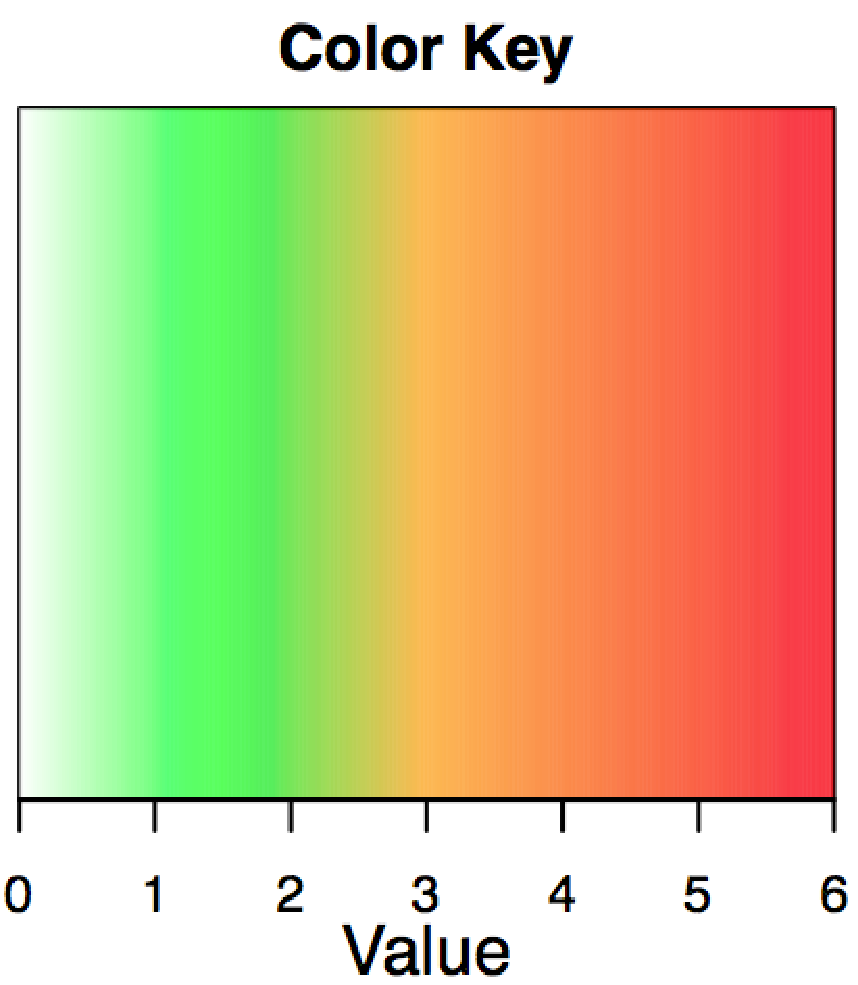
\includegraphics[width=.5\linewidth]{figures/heatmaps/colour-keys.pdf}
    \label{fig:hm-colourcodes}
  \end{subfigure}%
  \begin{subfigure}{.5\textwidth}
    \centering
    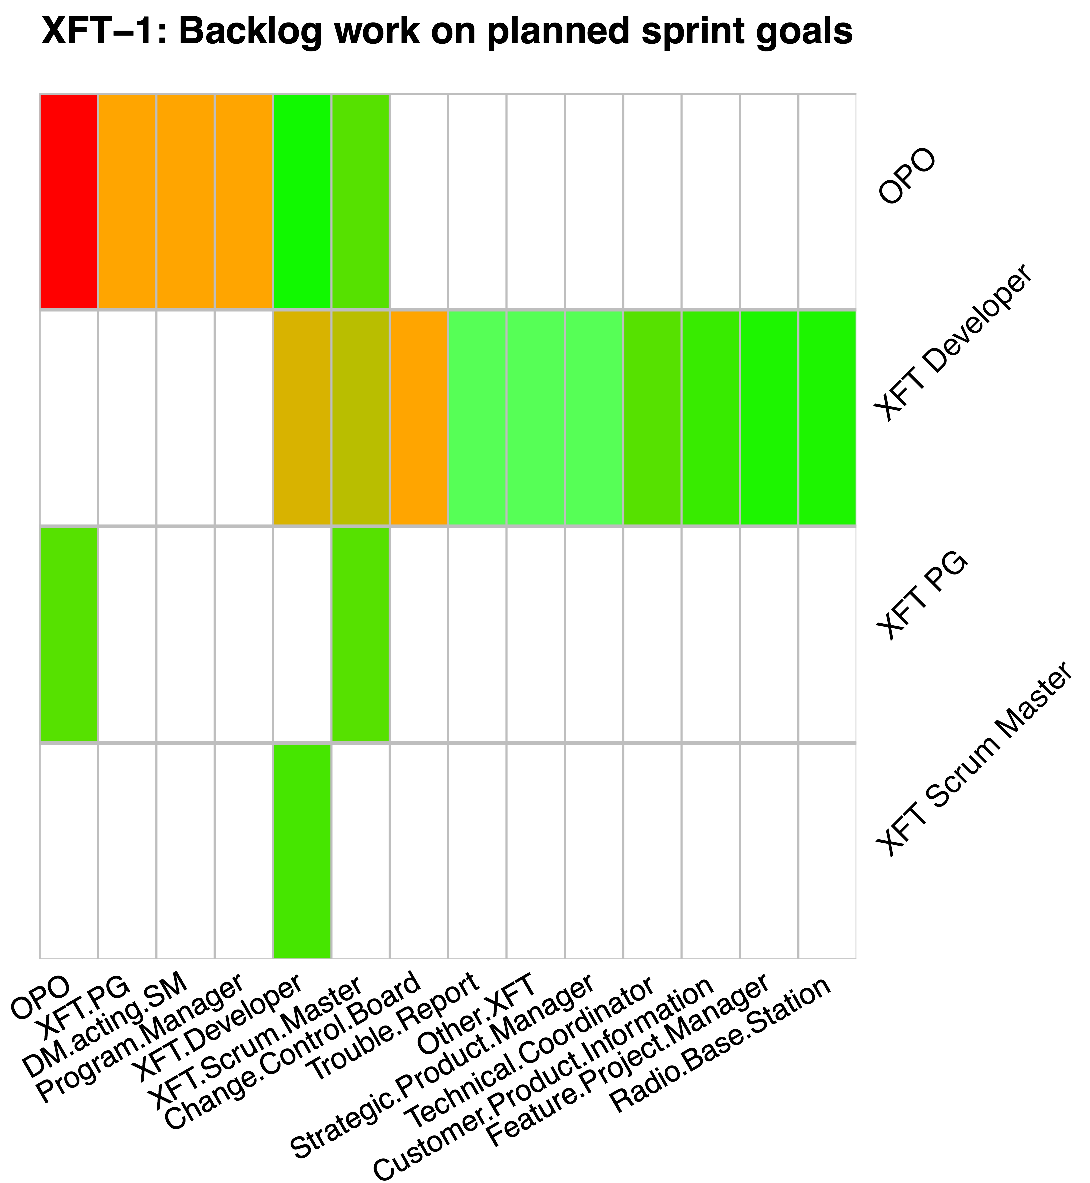
\includegraphics[width=.85\linewidth]{figures/heatmaps/ms2-_b_.pdf}
    \label{fig:hm-b-ms2}
  \end{subfigure}
  \begin{subfigure}{.5\textwidth}
    \centering
    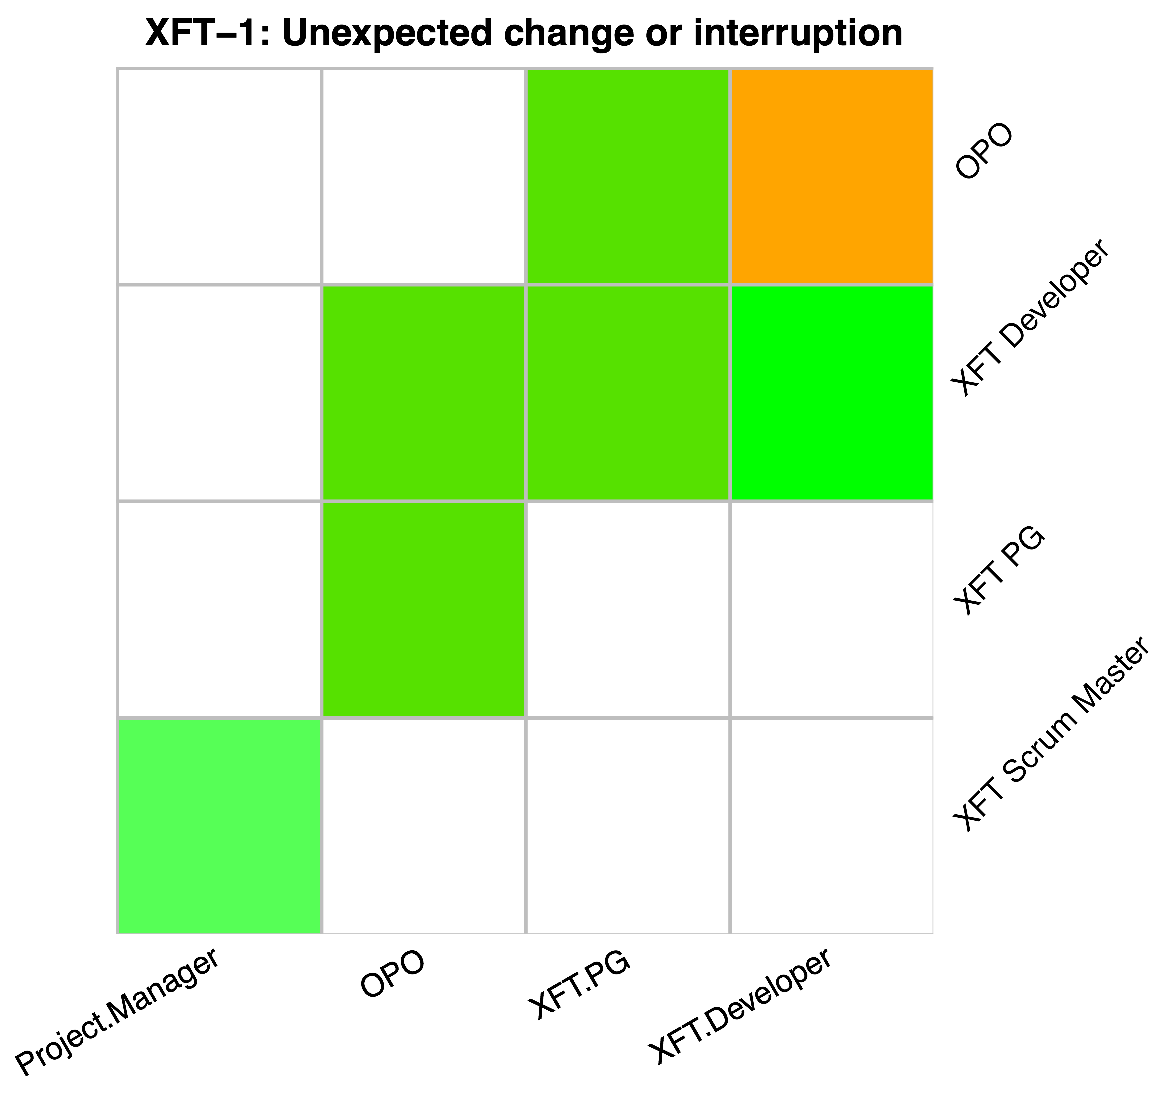
\includegraphics[width=.91\linewidth]{figures/heatmaps/ms2-_u_.pdf}
    \label{fig:hm-u-ms2}
  \end{subfigure}%
  \begin{subfigure}{.5\textwidth}
    \centering
    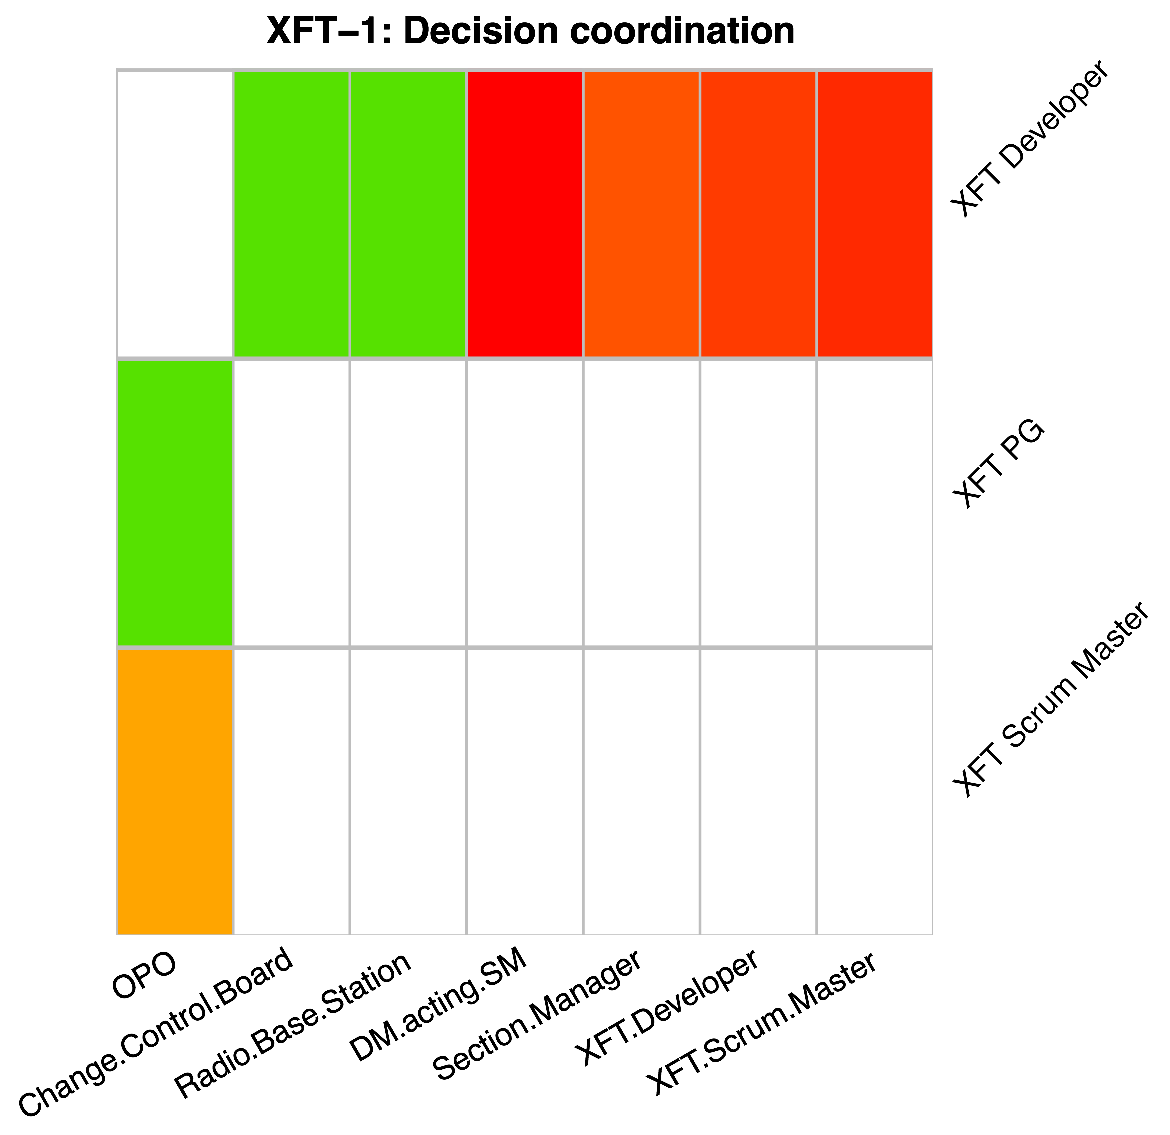
\includegraphics[width=.91\linewidth]{figures/heatmaps/ms2-_d_.pdf}
    \label{fig:hm-d-ms2}
  \end{subfigure}
  \begin{subfigure}{.5\textwidth}
    \centering
    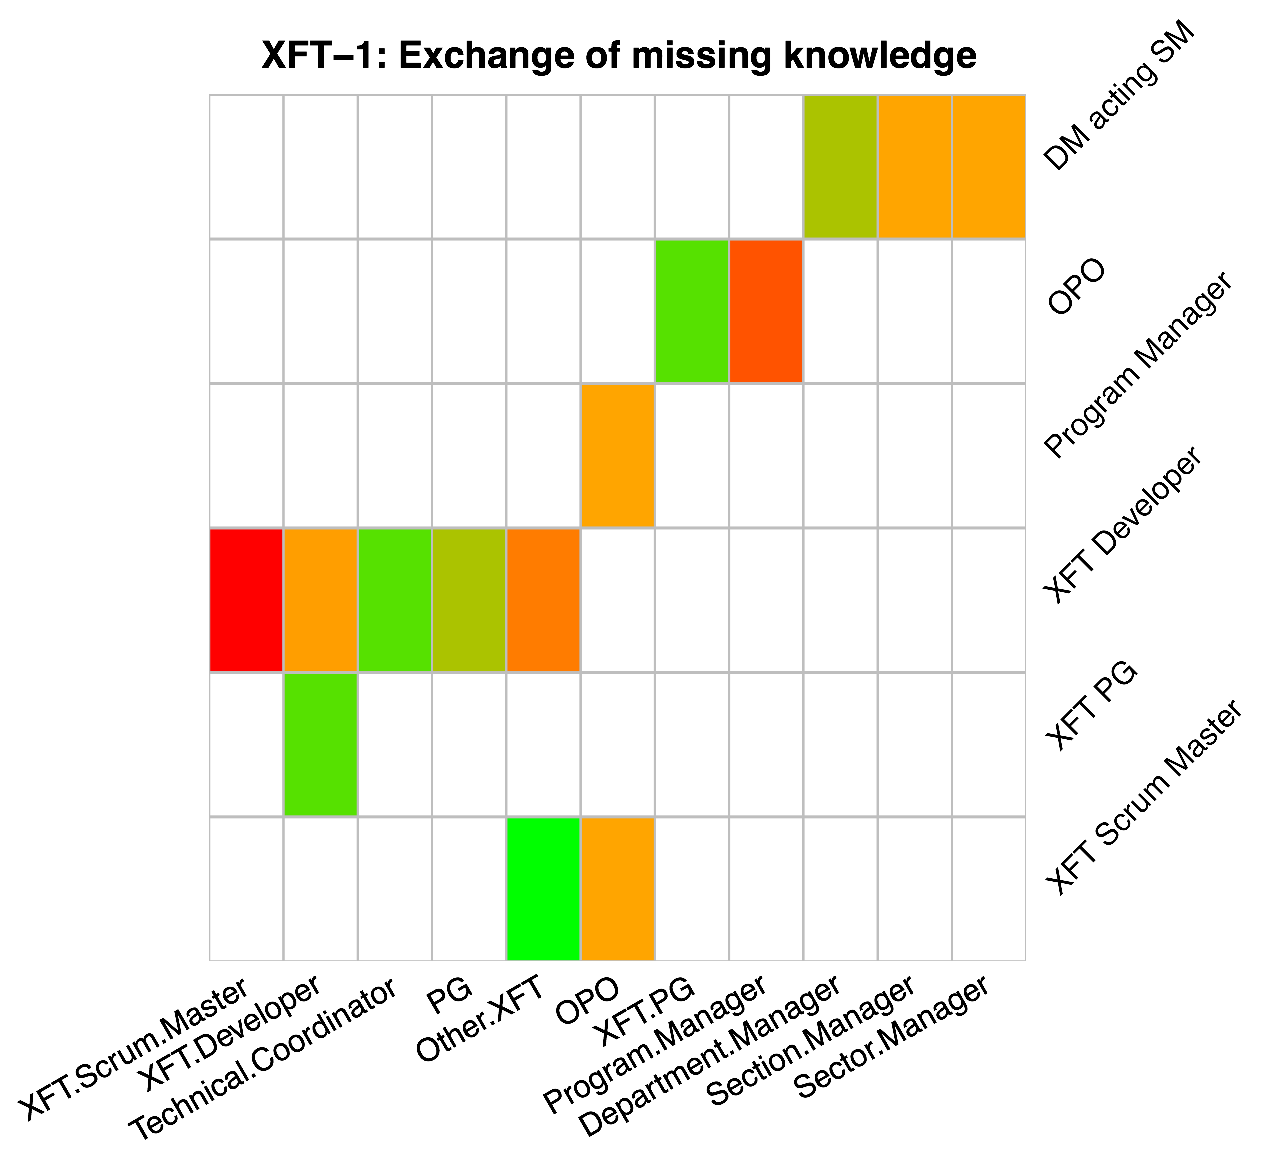
\includegraphics[width=.91\linewidth]{figures/heatmaps/ms2-_e_.pdf}
    \label{fig:hm-e-ms2}
  \end{subfigure}%
  \begin{subfigure}{.5\textwidth}
    \centering
    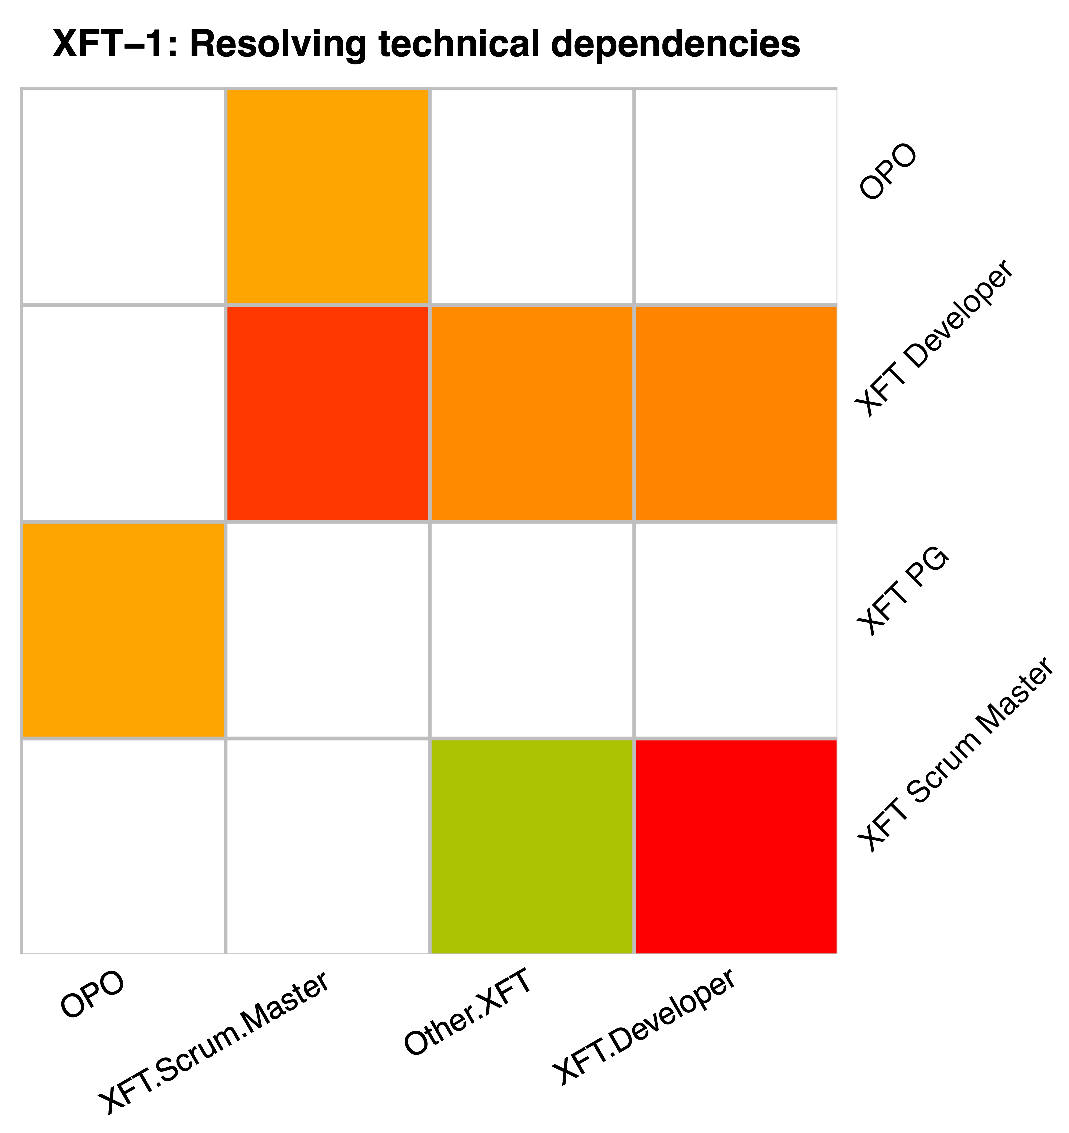
\includegraphics[width=.81\linewidth]{figures/heatmaps/ms2-_r_.pdf}
    \label{fig:hm-r-ms2}
  \end{subfigure}
  \caption{XFT-1: Differences in intensities depending on communication nature}
  \label{fig:hm-overall-ms2}
\end{figure}

\subsection{XFT-1 Heat Maps}
\label{sec:findings-xft1-hm}
As it can be seen from the Figure \ref{fig:hm-overall-ms2}, the most communication for the developers of the \ac{XFT}-1 is caused by backlog work, however they prevailingly considered it to be below the usual level of intensity. This is illustrated by the cells' colours being of varying shades of green which corresponds to the colour key's values below 3 --- a designator of the usual level (as in the case of communication of \quotes{XFT Developer} to \quotes{Change Control Board}). In contrast, \emph{Decision coordination} for developers more often involved communicating more intensively (note the red shades of colour codes corresponding to the values above 4). \emph{Unexpected change or interruption} seems to be the least intense communication for the team and their \ac{OPO}. \emph{Resolving technical dependencies} in the majority of the cases causes communication furthest above the usual intensity. Only on one occasion, \quotes{\ac{XFT} Scrum Master} to \quotes{Other \ac{XFT}} members, is it slightly lower that the usual intensity level, depicted with a cell coloured in a shade of green in contrast to others being of orange or red shades.

\begin{figure}
  \begin{subfigure}{.5\textwidth}
    \centering
    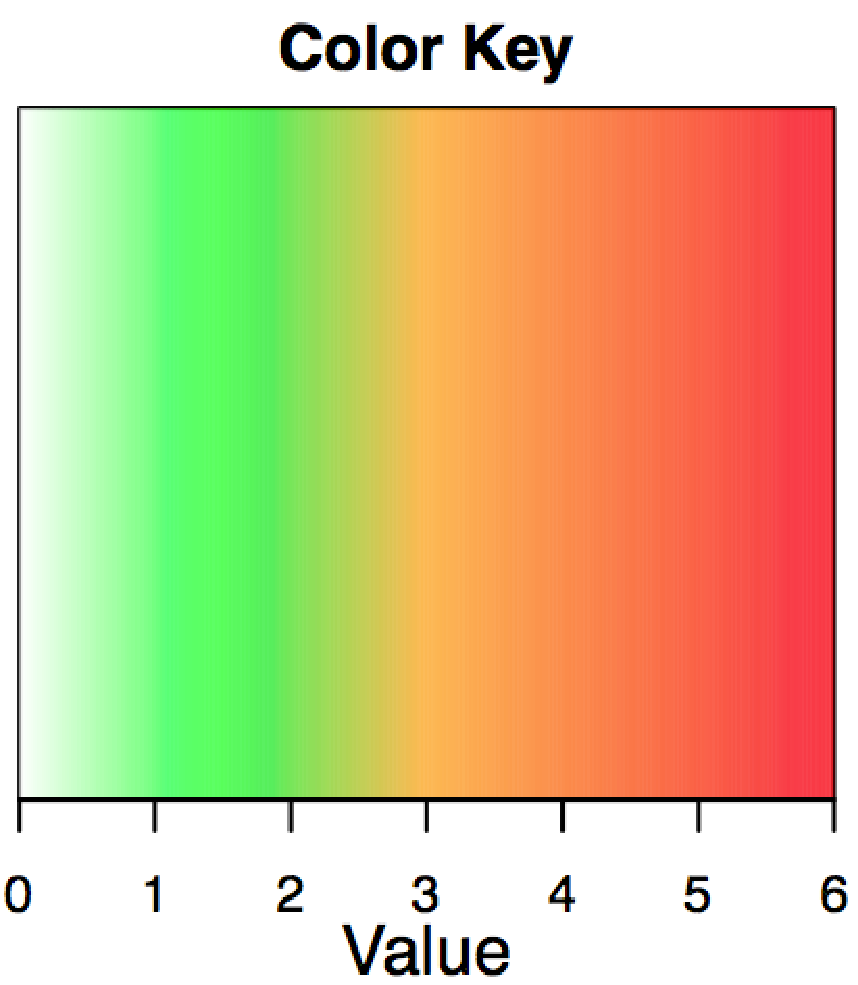
\includegraphics[width=.5\linewidth]{figures/heatmaps/colour-keys.pdf}
    \label{fig:hm-colourcodes}
  \end{subfigure}%
  \begin{subfigure}{.5\textwidth}
    \centering
    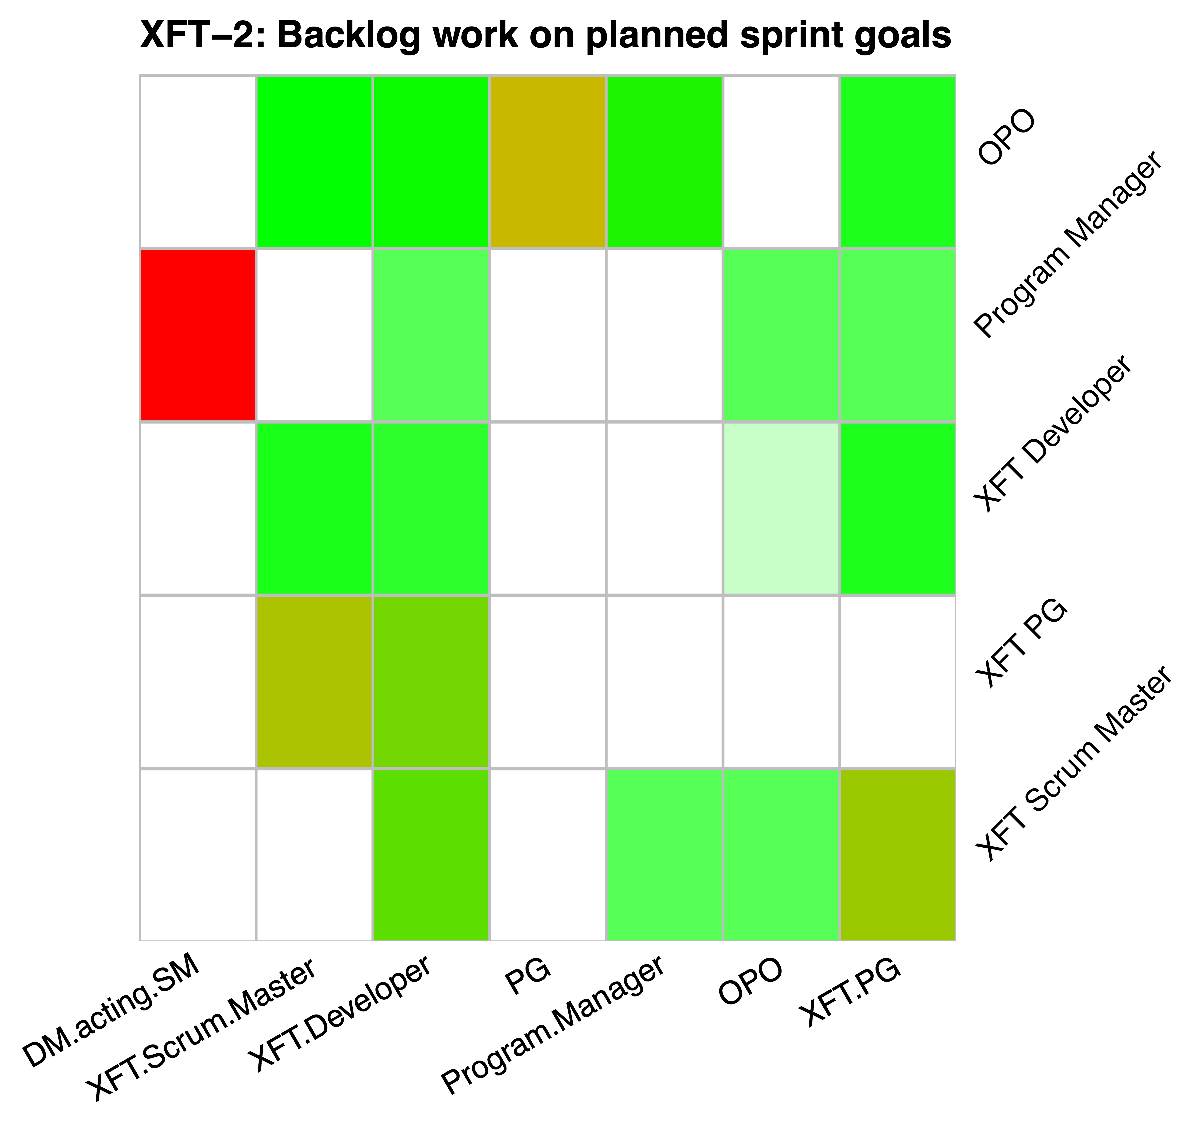
\includegraphics[width=.91\linewidth]{figures/heatmaps/picnic-_b_.pdf}
    \label{fig:hm-b-picnic}
  \end{subfigure}
  \begin{subfigure}{.5\textwidth}
    \centering
    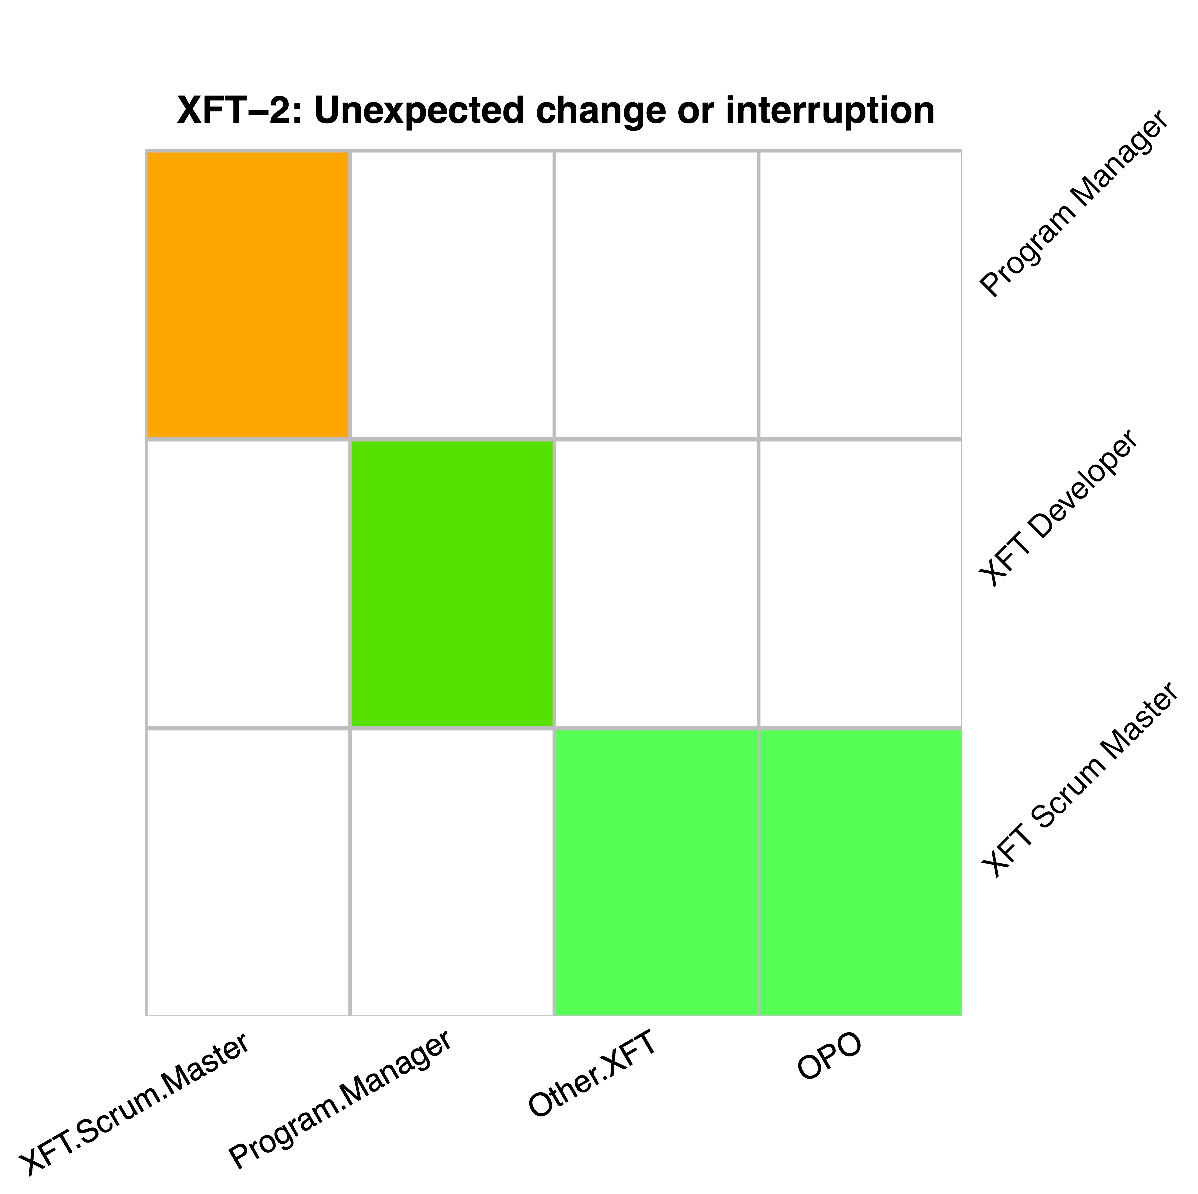
\includegraphics[width=.91\linewidth]{figures/heatmaps/picnic-_u_.pdf}
    \label{fig:hm-u-picnic}
  \end{subfigure}%
  \begin{subfigure}{.5\textwidth}
    \centering
    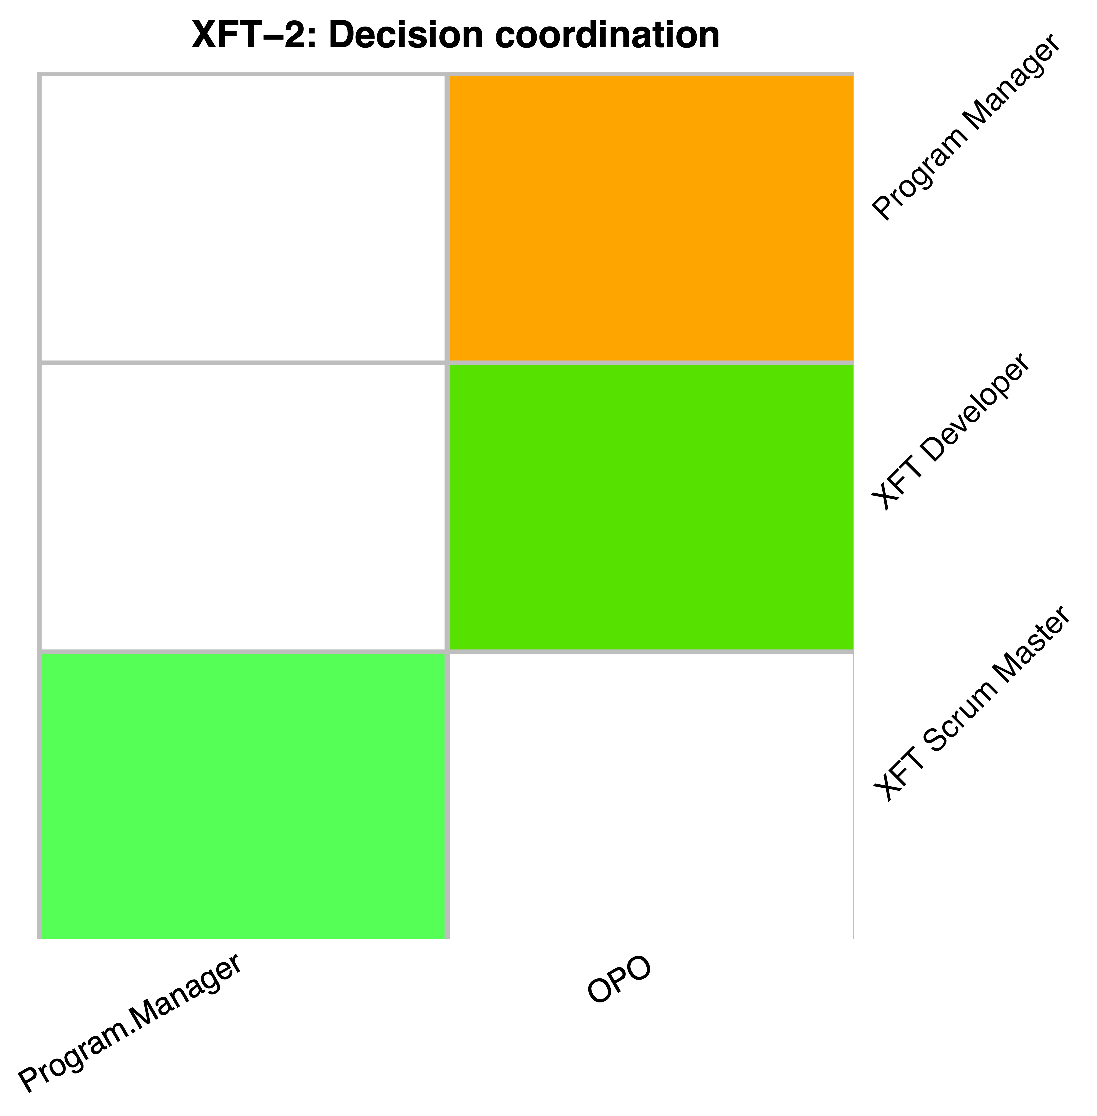
\includegraphics[width=.81\linewidth]{figures/heatmaps/picnic-_d_.pdf}
    \label{fig:hm-d-picnic}
  \end{subfigure}
  \begin{subfigure}{.5\textwidth}
    \centering
    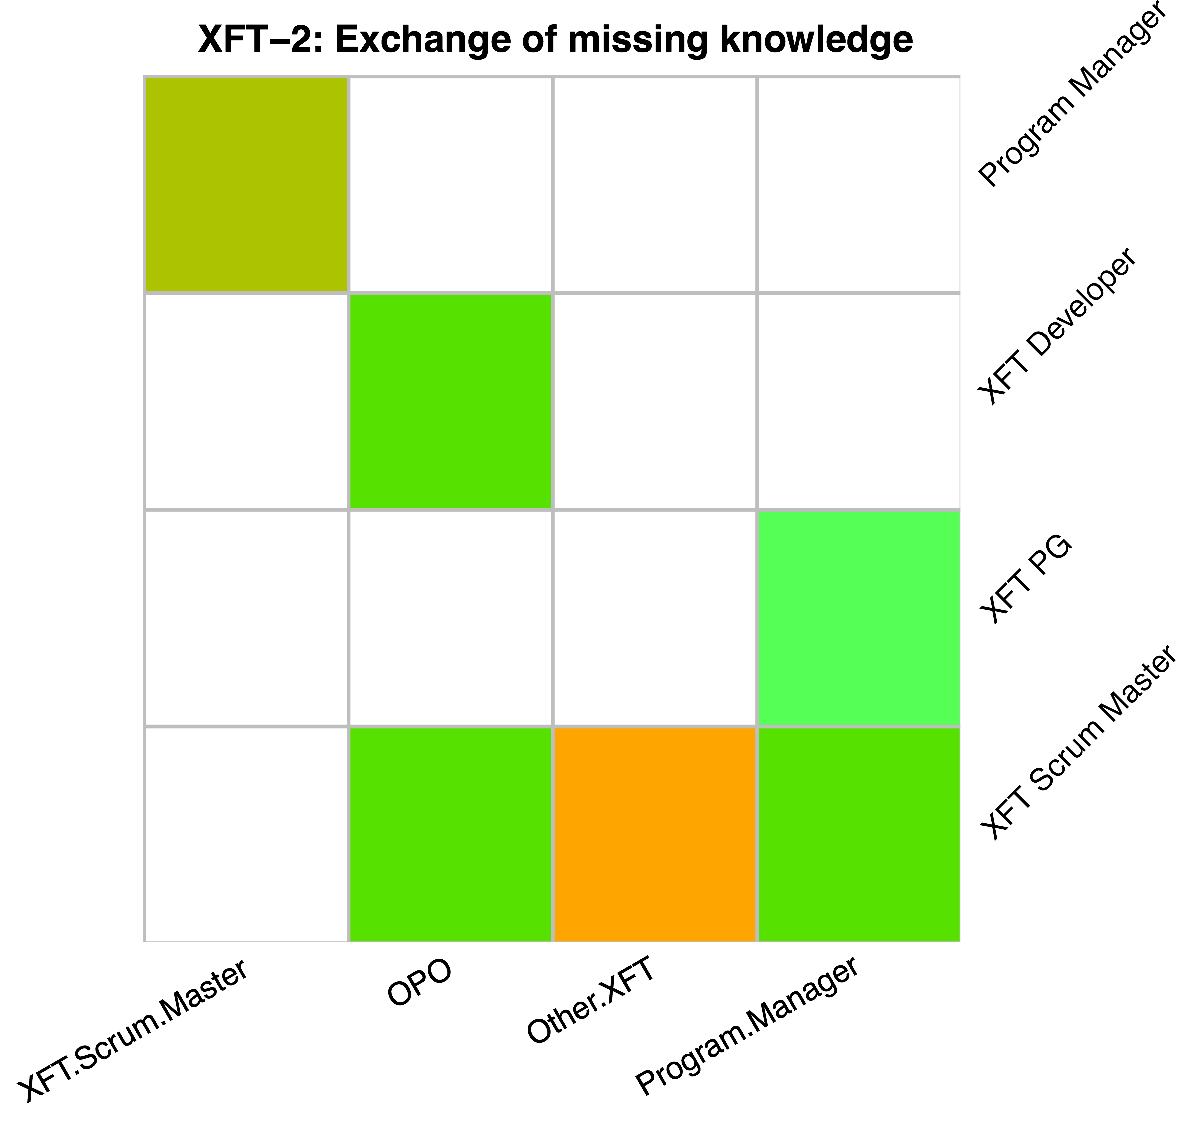
\includegraphics[width=.91\linewidth]{figures/heatmaps/picnic-_e_.pdf}
    \label{fig:hm-e-picnic}
  \end{subfigure}
  \begin{subfigure}{.5\textwidth}
    \centering
    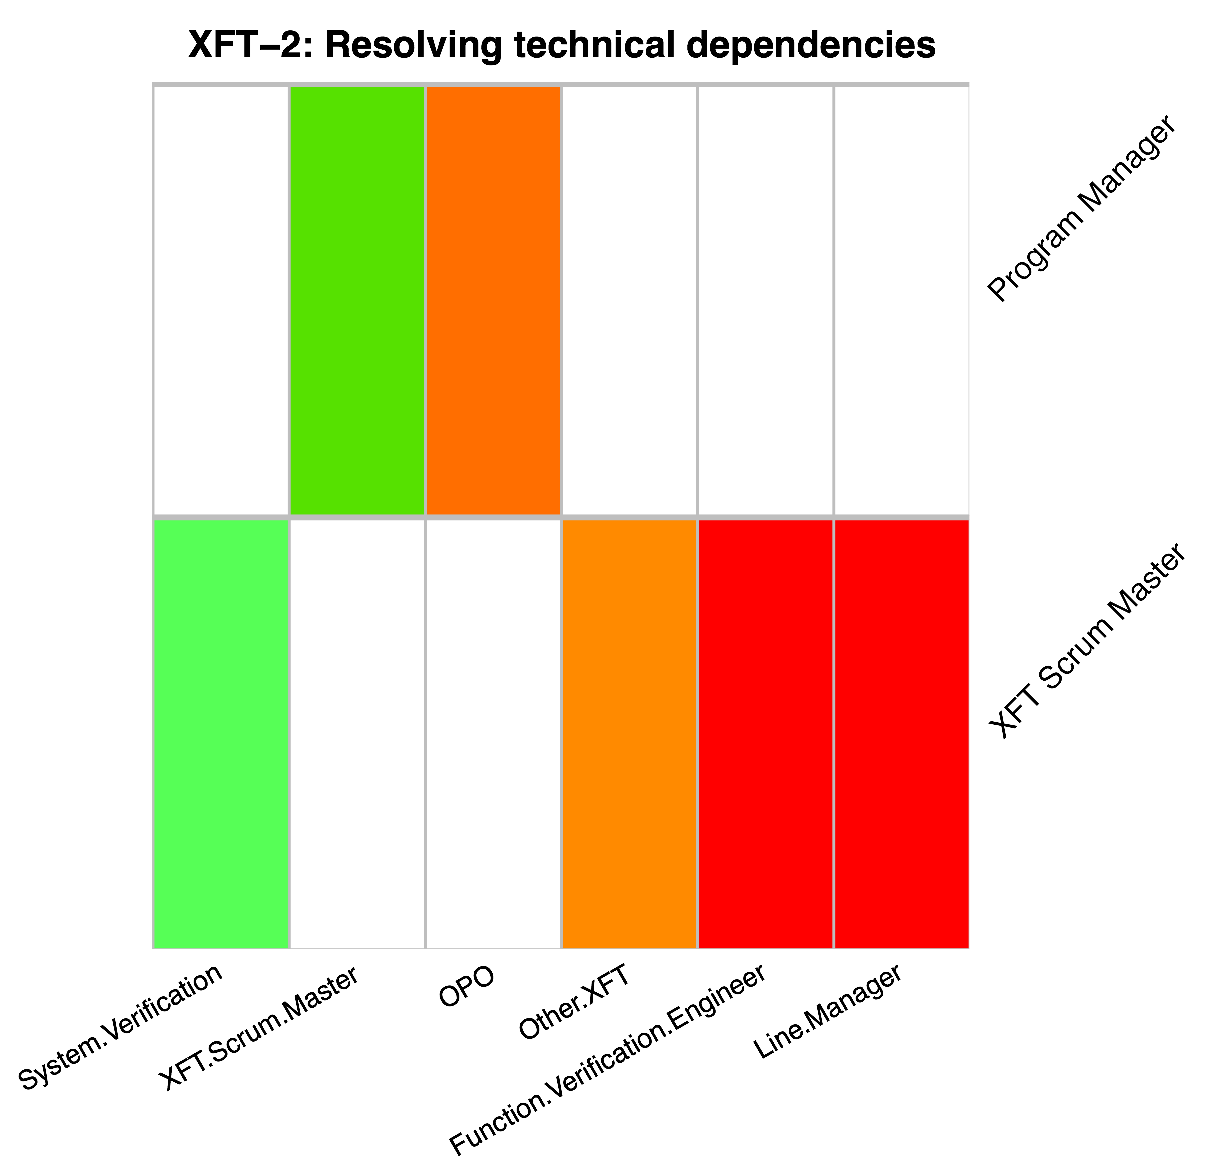
\includegraphics[width=.91\linewidth]{figures/heatmaps/picnic-_r_.pdf}
    \label{fig:hm-r-picnic}
  \end{subfigure}
  
  \caption{XFT-2: Differences in intensities depending on communication nature}
  \label{fig:hm-overall-picnic}
\end{figure}

Figure \ref{fig:hm-overall-ms2} also allows to observe how the roles present in heat maps change, depending on communication nature. The whole \ac{XFT}, the \ac{PG} and the \ac{OPO} have presence in all communication natures while the \quotes{Department (acting Section) Manager} and the \quotes{Program Manager} only step in for the \emph{Exchange of missing knowledge}. The survey allowed the respondents to mark "Other" as a communication nature. Although not visualised separately, it should be noted that the greatest part of communication of the \quotes{Program Manager} involved planning activities while the \quotes{Department (acting Section) Manager} to a great extent discussed the existing working set-up with his colleagues in the line organisation.

\subsection{XFT-2 Heat Maps}
\label{sec:findings-xft2-hm}
The week under study for the \ac{XFT}-2, visualised with heat maps on the Figure \ref{fig:hm-overall-picnic}, was (with a few exceptions) of a rather light communication intensity. The most popular communication nature was \emph{Backlog work on planned sprint goals} where, again, the intensity was mostly below the usual levels. As can be seen, only the cell depicting communication of the \quotes{Program Manager} with the \quotes{Department (acting Section) Manager} is colour-coded with red whereas the rest are of green colours corresponding to the levels of intensity below 3 --- a designator of the usual level. \emph{Unexpected change or interruption} along with \emph{Decision coordination} were only marked by the XFT members and the \quotes{Program Manager} and the intensity there never raised above the usual level.

Overall, a rather tight collaboration between the respondent group can be observed from all the heat maps on the Figure \ref{fig:hm-overall-picnic}. The \quotes{XFT Developers} mostly stayed within their immediate communicational environment of their \ac{PG}, \ac{OPO}, \quotes{Program and Department (acting Section) Manager}, with only the \quotes{XFT Scrum Master} reaching out in cases of \emph{Exchange of missing knowledge} and \emph{Resolving technical dependencies}. In addition to the \quotes{\ac{XFT} Scrum Master} being the only member of the \ac{XFT} involved in resolving technical dependencies, this communication nature caused the most intense interactions for him.

\subsection{Social Networks}
The data collected from the surveys was also used to construct social networks and thus give an overview of the interconnections between various roles in the studied groups of respondents.

The nodes in the social network graphs corresponding to the roles in the respondent group are indicated by the nodes of a bigger size. The representatives of the \quotes{XFT-D} role in the network on the Figure \ref{fig:ms2-sn} participated in the study by filling out the surveys while the representatives of the \quotes{TC} role did not and were only approached by \quotes{XFT-D} over the studied period. The amount of new roles increases from the heat maps to social networks. This is explained by the fact that the respondents were able to mark "Other" as a communication nature and thereby this communication was not included in any of the heat maps, as it has been mentioned above.

\begin{figure}[h!]
  \centering
  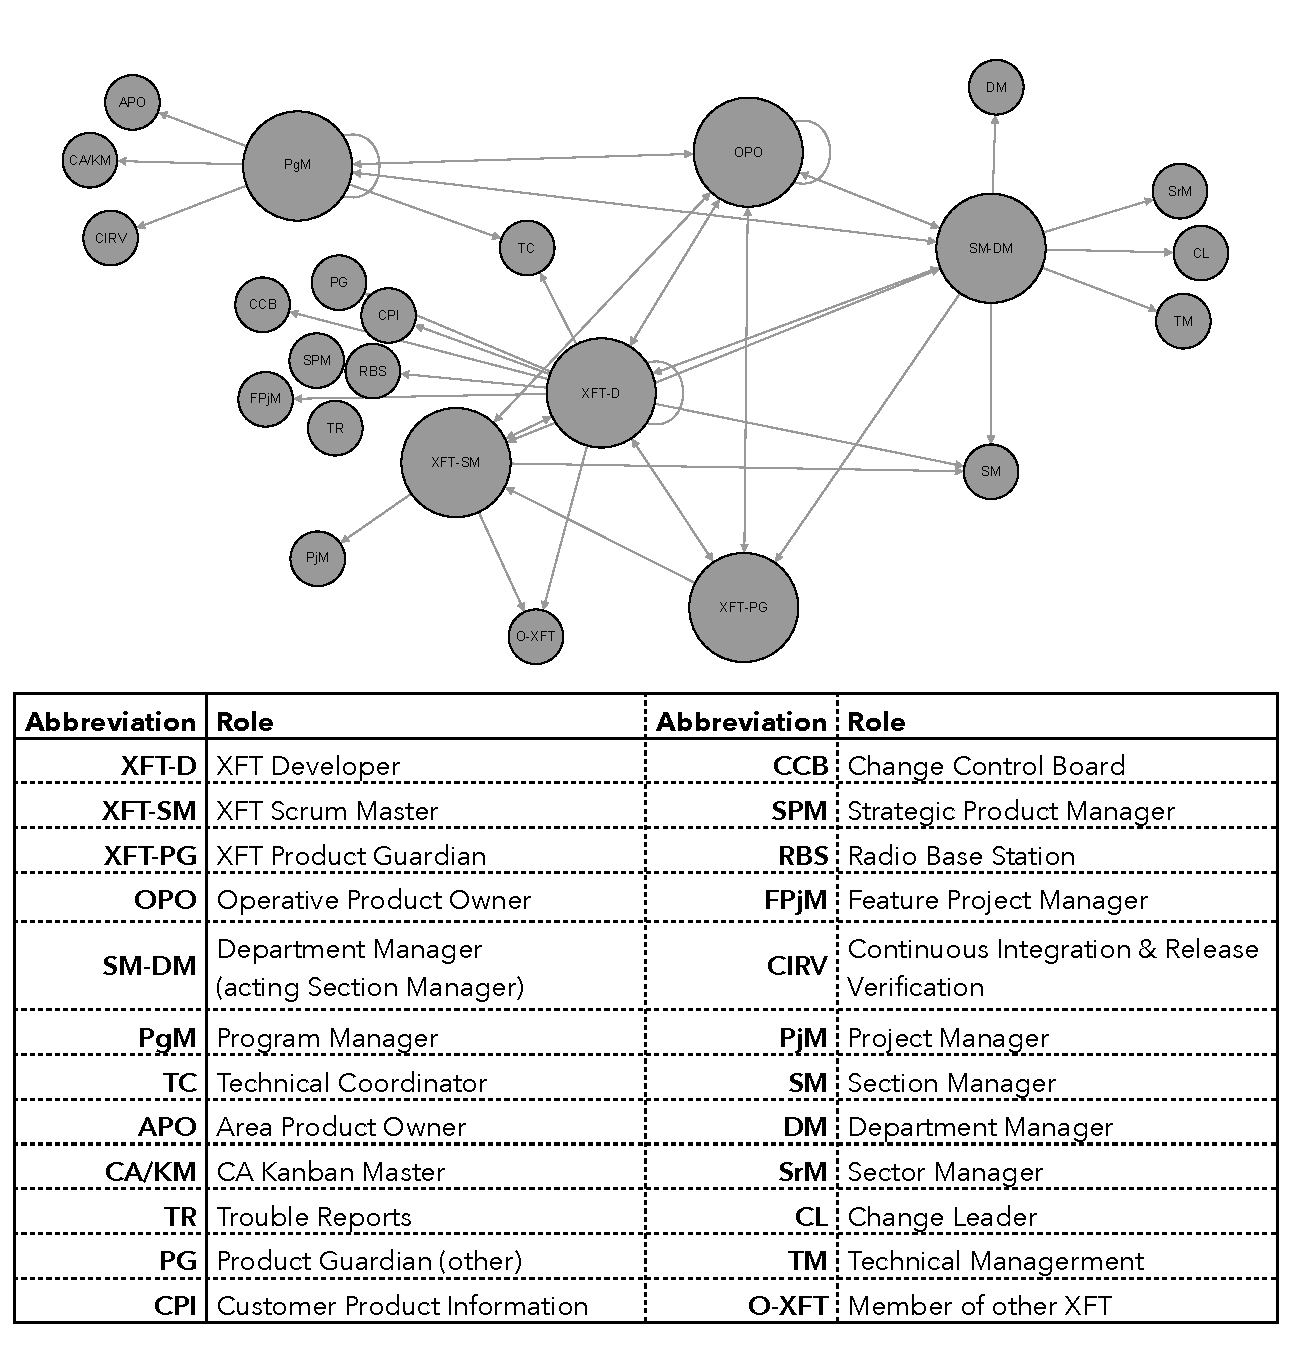
\includegraphics[width=1\textwidth]{figures/sn/sn-ms2-legend.pdf}
  \caption{XFT-1: Social Network}
  \label{fig:ms2-sn}
\end{figure}

The social networks characterisation of communication patterns of both teams is depicted in the Figures \ref{fig:ms2-sn} and \ref{fig:picnic-sn}. Close collaboration between the members of the \acp{XFT} and their \acp{OPO} and \acp{PG} is attributable to both teams, which is a positive finding in the context of desired collaboration layers illustrated on the Figure \ref{onion}. The communication between the \acp{XFT} and their \quotes{Section Manager} in both cases has been found to be less tight. Although connected in the networks, these roles seem to have rather limited collaboration based on the heat maps tables. As has been mentioned in sections \ref{sec:findings-xft1-hm} and \ref{sec:findings-xft2-hm}, both have only been in contact over decision coordination in the case of \ac{XFT}-1. Still, the teams communicated with their \quotes{Section Managers} during meetings.

Over the course of one week, the members of the \ac{XFT}-1 had connections to ten roles who are not part of their immediate environment, as shown on the Figure \ref{fig:ms2-sn}. Most of them were initiated by the developers rather than the \quotes{\ac{XFT} Scrum Master}: nine out of ten for the former and two out of ten for the latter with a single overlap. The \quotes{Program Manager} of the \ac{XFT}-1 is rather detached from the team with communication flowing via the \quotes{\ac{OPO}}. The \quotes{Department (acting Section) Manager}, although connected with all members of the respondent group, has an equal number of communication with other roles mainly from the line organisation. Referring back to the heat maps calls for a conclusion that the latter set of communication paths is of a greater significance for the role.

The social network of the \ac{XFT}-2 overall has notably less connections than its counterpart, possibly due to the internal nature of the tasks at hand. Here, the team is in collaboration with their immediate environment. However, similarly to the \ac{XFT}-1, the \quotes{Department (acting Section) Manager} is connected to all respondent roles but as can be tracked from the heat maps, the contacts between them are not frequent. The \ac{XFT}-2 has six contacts with the roles outside their immediate environment, with the \quotes{XFT Scrum Master} contributing the most and solely having five of them. Thus, outside communication to a great extent seems to be flowing via the \quotes{XFT Scrum Master} who acts as a communication hub.

\begin{figure}[h!]
  \centering
  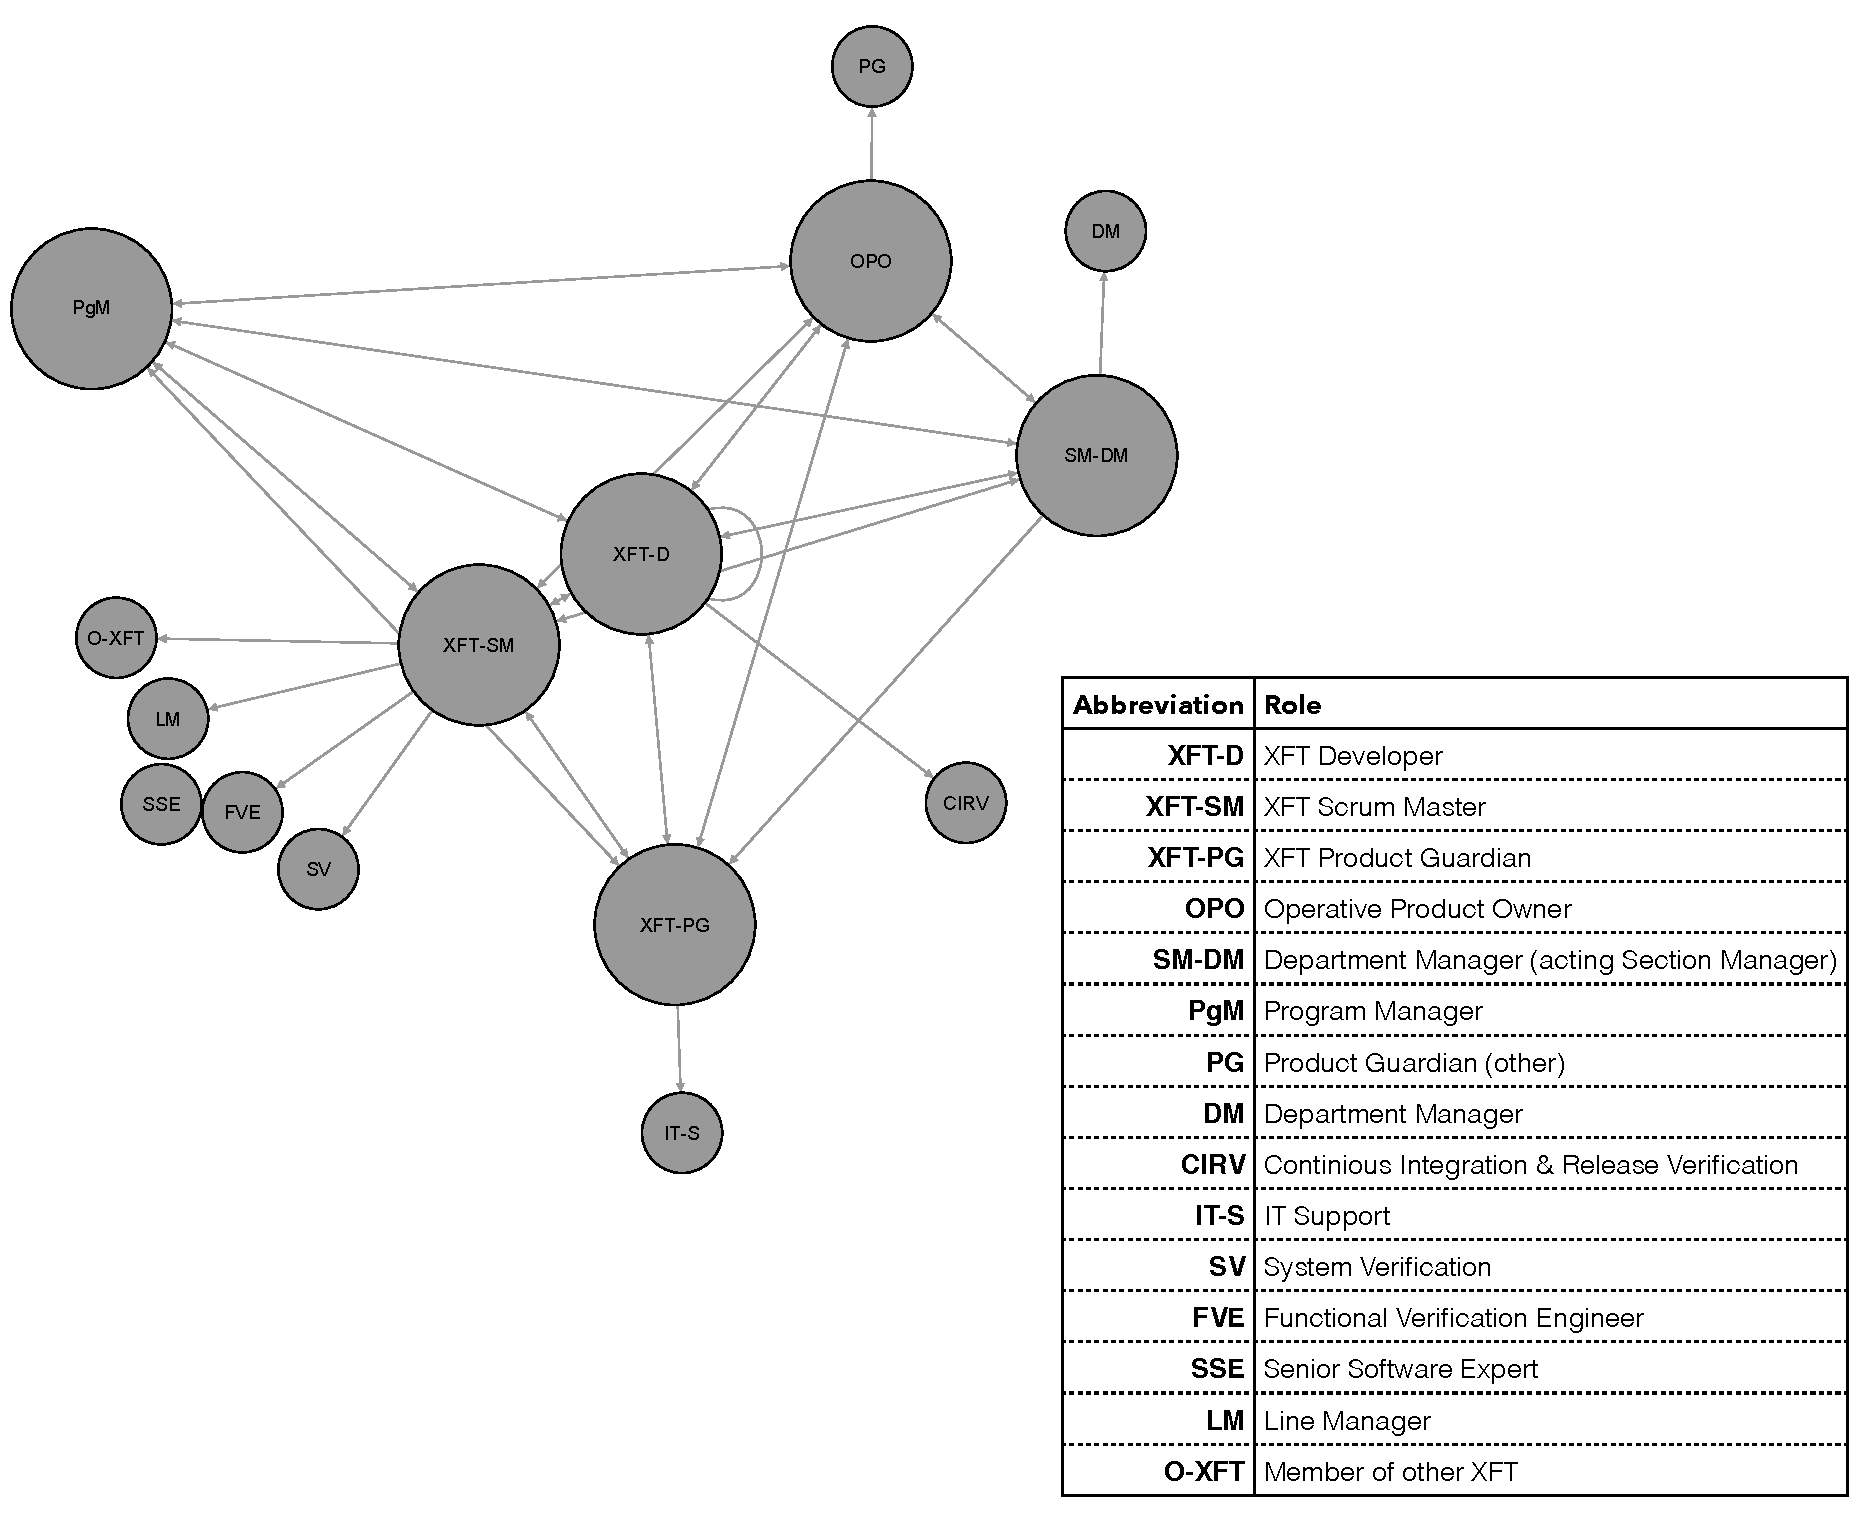
\includegraphics[width=1\textwidth]{figures/sn/sn-picnic-legend.pdf}
  \caption{XFT-2: Social Network}
  \label{fig:picnic-sn}
\end{figure}

\section{Information \& Communication}

The analysis of the daily surveys was followed by the analysis of the interviews' data. This section focuses on the data discovered in connection to the first research question.

\textit{\textbf{RQ1:} What are the information and communication challenges associated with the adoption of large-scale agile and how does their resolution benefit the application of agile?}

The findings are divided as pertaining to either information or communication as defined in Section \ref{chap:background-comm-info}.
They are organised in three groups: challenges, benefits and improvements. The challenges describe the existing problematic aspects of information and communication flows while benefits picture desirable situations that could foster interviewees' work. The improvements suggest means of overcoming the challenges and thus reaping benefits, however it should be noted that these are solely the opinions of the study's participants which might favour transitions from challenges to benefits, but are by no means complete and capable of solving all of the existing problems.

All findings are illustrated with quotes from interviews transcriptions. Naturally, the amount of quotes for each finding does not reflect their magnitude. The excerpts of opinions are rather used to describe an issue from several perspectives where applicable.

\subsection{Information}

The findings related to the concept of information are summarised on the Figure \ref{fig:information}.

\begin{figure}[h!]
  \centering
  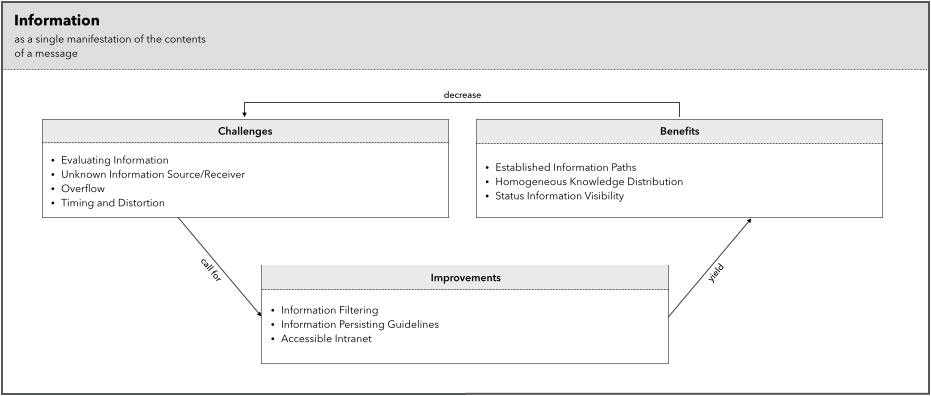
\includegraphics[width=0.98\textwidth]{figures/information.png}
  \caption{Information challenges, benefits and improvements}
  \label{fig:information}
\end{figure}

\subsubsection{Challenges}

\begin{description}

   \item[Evaluating Information.] Each XFT in the studied organisation follows their own development process. From the interviewees' point of view it is favourable to have access to the descriptions of thereof. This can serve as a source of inspiration for own process improvements or assist in solving problems that might have been encountered previously by another team. However, the information circling around the organisation does not undergo a strict evaluation process, according to the interviewees. This leads to situations where the same issue is described in several different ways which differ significantly. For the people seeking this information it is troublesome to sort out approved pieces of it. The interviewees emphasize a need of reliance on the information that is commonly accessible by every party within the organisation.
   
      \begin{quote}\itshape ... we say that \quotes{We have decided that we will do this and this and that" — that is not so easy to find, because you could find 10 "We have decided this and this and that} so which one is valid? ... It should be more clear about that kind of information, what kind of information is approved and which is not. Because we really can't afford to run on information that is not valid.
      \end{quote}

   \item[Unknown Information Source/Receiver.] Although acknowledged as a fundamental and integral activity of each organisational unit, information sharing remains an intricate problem, which consequently adds to the problem of information gathering. Due to a not always clear separation of responsibilities, information is often being broadcast to every party that may, according to the information source, be interested thus leading to big amounts of "so that you know" information spread. At the same time, those who are genuinely in need of this intelligence and would benefit from it are potentially left unaware.
      
   The organisation uses an internal portal to store information that is accessible by the employees. By means of this portal, teams can put up status updates or share information pertaining to their work. Still, while diligently updating their Wiki pages, the respondents mark that the information is not reaching its' seekers due to unstructured nature of the portal that makes the links hard to find.

      \begin{quote}\itshape Of course it's visible for more or less everyone, but I know for myself that if I enter another area, it's really tricky to find if I don't have any clues about where to start searching.
      \end{quote}

   Consequently, information gathering demands a significant effort. Whenever~\acp{XFT} are being faced with an unknown domain in their work packages, they are lead to dead ends with a need for information hunting also not knowing where to begin the search.

   Unclear responsibility concerns negatively affect the information gathering process as well, creating unnecessary long information search paths.

      \begin{quote}\itshape Many times I would like to just know "Who do I ask?". I mean I could ask one person just to get the name of the person who I really should ask to find out for a specific thing.
      \end{quote}
      
   These situations make~\acp{XFT} reliant on their personal social networks that have been established while working at the organisation. Information discovery in these networks is accidental rather than the information flow building up the evidence.

      %\begin{quote}\itshape ... I got the information that this team over there is working on something that is you do, because I’ve met that guy at the coffee machine and as I knew him from before I had a discussion. So it is depending more on your personal relationships with persons around in the organisation than on actual information flow.
      %\end{quote}

   \item[Overflow.] A problem of an overwhelming amount of information constantly circulating within the organisation was noticed by almost every interview participant and is one of the most prominent challenges. The interviewees mentioned numerous E-Mails reaching them on a daily basis from a vast variety of sources, which span across work-related issues, inquiries to provide competence and variety of newsletters from different parts of the organisation. In addition to this, there are numerous demo events and synchronisation meetings. The incomprehensible flow of incoming data is hard to handle without loosing the focus of one's primary work and thus leads to either unnecessary long data acquisition engagements or ignoring the potentially relevant information.
   
      \begin{quote}\itshape ... if you get a lot of emails each day, a lot of them you can’t read by physical limitations — you have to throw them away. Sometimes you miss stuff. It’s a lot of stuff but sometimes you miss the important.
      \end{quote}

   \item[Timing and Distortion.] In an environment which requires agreements from several parties to proceed on a certain task, it is not always possible to hold a common discussion at the same time. This creates the need for several coordination meetings sometimes parted by a number of days where information clutters and spreads thus disrupting the atmosphere around the~\acp{XFT}.
      
      \begin{quote}\itshape ... you have this distorted information and some team has heard something and some team has not. And then when it involves some kind of change then people don't really know what to trust.
      \end{quote}

\end{description}

\subsubsection{Benefits from Overcoming Challenges}

Unimpeded and fluent access to information will smooth the working environment of \acp{XFT} by reducing the time needed for the information search, promoting knowledge sharing and shifting the focus of the developers to their primary backlog work.

\begin{description}

   \item[Established Information Paths.] A structured information flow within the organisation will contribute to a resolution of information overflow and consequent problems. Establishing communication paths comes with a significant cost by the need to sort out all existing information sources and declare paths to access them while at the same time saves the information that potentially could be lost due to misguiding travel paths.
   
   %\begin{quote}\itshape Sometimes the same information travels and sometimes into different speeds and sometimes information is only flowing one path. So that's where we sometimes end up in situations sometimes we don't really understand what happens different sides.
      %\end{quote}

   \item[Homogeneous Knowledge Distribution.] Having a clear structure of the information flow within the organisation will help information to reach its intended audience. By removing the unclarity of intended information sources and receivers, knowledge will spread more fluently and evenly, meaning that the chances for each person to get access to the same piece of information are more or less the same. This homogeneous distribution of knowledge assists, for instance, promoting the adoption of best practices between several teams and reducing the amount of double work.

   \item[Status Information Visibility.] Availability of information regarding the status of work in a collaborative environment is crucial to successfully determine a project's health. The benefits of having unimpeded access to status information at all times are two-fold: while the information source is shielded from being disrupted when such information is requested, information seeker is not dependant on availability of information provider. Thus various units in the organisation are allowed to follow up on each other without significant effort.

%\begin{quote}\itshape ... most of the managers are team coaches for the teams but the other managers don't have that information for other teams. They only have information regarding their own teams. Also I have no time to walk around for every team and be a part of their daily Scrum. So it's good for me to also have a very short slot of every team every day so I can easily pick up if there is any problem with the teams.
 % \end{quote}

\end{description}

\subsubsection{Potential Improvements}

\begin{description}

   \item[Information Filtering.] An ability to filter out incoming information is desirable to overcome the information tsunami~\acp{XFT} are faced with. While some interviewees suggest to mission a specific role for selecting information that is valuable for the teams, others propose the creation of seeking profiles for better customisation of heterogeneous needs of different roles with varying areas of concerns.
   
   \begin{quote}\itshape I think the teams need to do that themselves really, because its better to have information available but then everyone has a bit different needs. It's better that they do their own seeking profile than someone plans it for them.
   \end{quote}

   \item[Information Persisting Guidelines.] The respondents seem generally concerned about the faultiness of the existing way of spreading information. The seeming anarchy caused by the lack of a commonly agreed and followed rules regarding information persistence leads to the knowledge being lost inside the teams as they do not know a ways of sharing it or being lost in a sea of unevaluated information not easily reachable by others. The interviewees expressed the need of information persisting guidelines while marking the importance of knowledge sharing practices.
To decrease the amount of unreliable data one proposal, for instance, was to include a review step prior information persistence, where the suggestions are analysed and their validity is evaluated. 
   
   %For instance, one interviewee describes a possible way of approaching information evaluation before its persistence:
  
  %\begin{quote}\itshape Tips \& tricks, everybody should be able to put up stuff there in order to collaborate better and "Well, try this one out. I tried and it worked". Of course that's good, but we also need to evaluate that, to have some parts that should be a little bit more stiff to change. I'm not meaning that it should be completely stiff, but they should be a little bit more so that you kind of make a suggestion and some people are reviewing this suggestion and say "This is good, lets put it in", not just putting in all the stuff that everybody comes up with.
   %\end{quote}

   \item[Accessible Intranet.] An Intranet is capable of providing access to all of the shared information while at the same time it lacks a comprehensible structure. The interviewees note the discouragement of using it as an information platform as it simply does not have a common entry point. Reshaping it in a way allowing for information filtering will contribute to a more thorough use and a clarification of ways of information sharing.
   
\end{description}

\subsection{Communication}

To recall, the thesis makes a distinction between the concepts of information and communication, where the latter is a form of humans dynamically exchanging information while the former is viewed as a single manifestation of a message content thus representing a more static concept.

The findings on the communication aspect of the first research question are summarised on the Figure \ref{fig:communication}

\begin{figure}[h!]
  \centering
  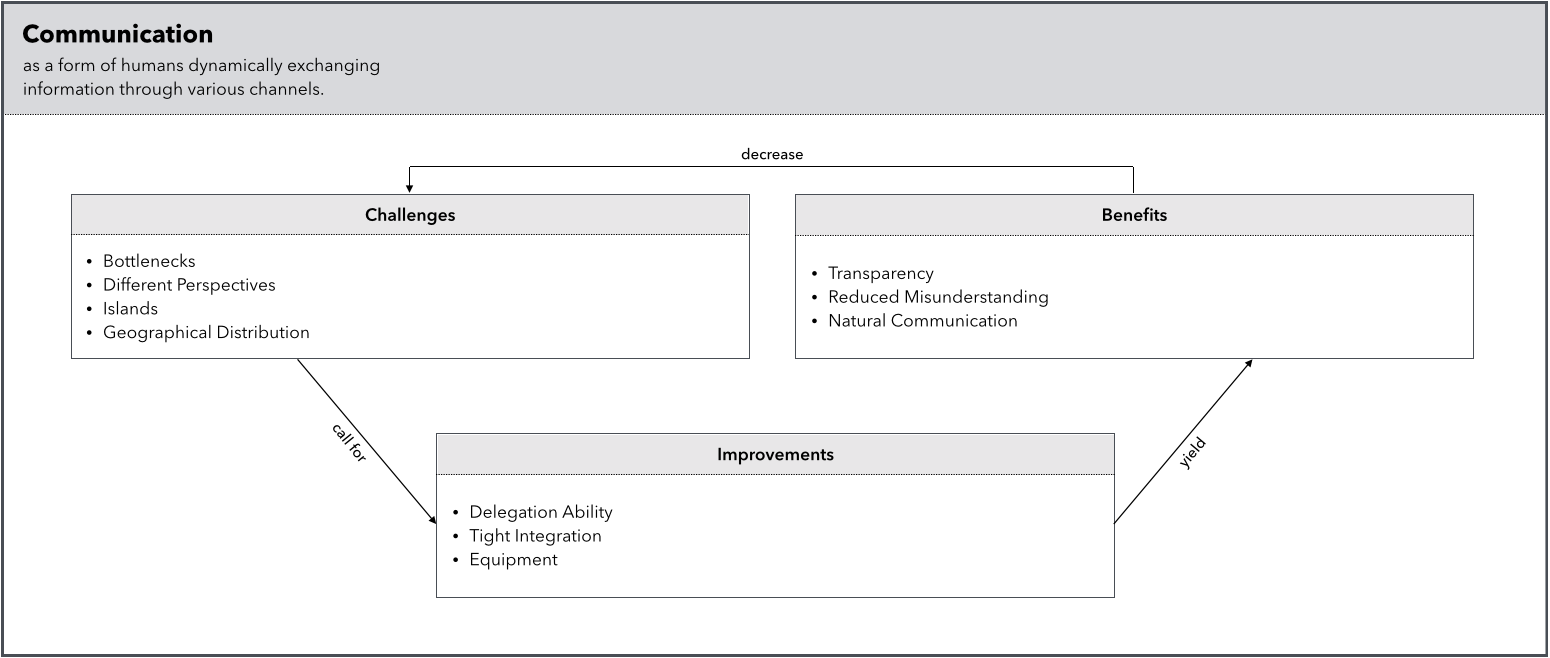
\includegraphics[width=0.98\textwidth]{figures/communication.png}
  \caption{Communication challenges, benefits and improvements}
  \label{fig:communication}
\end{figure}


\subsubsection{Challenges}
\label{subsubsection:comm-chall}

\begin{description}

   \item[Bottlenecks.] Having a growing organisation of a large-scale comes at a cost of required extra coordination by several roles and persons exclusively holding responsibilities or information needed by a variety of units. Apart from bringing heavy load on the bottlenecks themselves it creates delays for dependant parties.
   
      \begin{quote}\itshape They have very-very many features to keep track of, but when something arise and get very hot, they are coming back, but if it's not that hot it takes long time, because they have such a full load on that.
      \end{quote}

   \item[Different Perspectives.] Due to differences in day-to-day concerns interviewees are faced with in their work, it is not uncommon that communicating instances diverge in their levels of attainment with various topics. This leads to misunderstandings that can turn into hindrances for either of involved parties. Different perspectives and levels of understanding of a task may invoke confusion for one of the ends of a communication channel as it hinders assessment of impact on their work.

      %\begin{quote}\itshape %It’s very difficult to get feedback if you have people understood. Because it’s all about understanding.
      %The problem is that the Project Manager sees it very clear, the goal, but for me it’s not clear. You say something like that, but the impact on my work — I have no idea.
      %\end{quote}
      
   Some of the interviewed developers note that sometimes they are being enforced to take part in time consuming, not beneficial communications, stemming from the fact that the organiser of the meeting, likely unintentionally, misjudges its usefulness for different participants:

      \begin{quote}\itshape You have a different point of view form a Project Manager. When he calls that meeting he has a status from all the teams, but that team does not care at all what this team does, so the benefit is only for the Project Manager, mostly.
      \end{quote}

   \item[Islands.] A concern cross-cutting through several interviews is the presence of communication islands. These are shaping around certain roles who tend to have the greatest deal of the daily encounters with a limited number of other roles. This results in knowledge concentration and its' following isolation inside these emerged groups. The interviewees mentioned this phenomena as both positive and negative aspect of the existing communication set-up thus supporting the challenging nature of balancing it out.
   
Small numbers of teams working on the same product have been mentioned by the interviewees as a beneficial factor for~\acp{XFT} due to close connections with other teams — they are contributing with a clear separation of work and provide availability of competences on other parts of the product the team is reliant on.

      \begin{quote}\itshape We are three teams working with [product], it's very good functioning and we are all focused in one product. We are also situated in one area, so there are good communications between those 3 teams that is no issues at all.
      \end{quote}

   On the other hand, such a separation from the rest of the organisation has the drawback of missing out on work and ways of working in other teams.

     % \begin{quote}\itshape But since we are sitting in that area we don't really have that much knowledge about other, how are other teams working.
      %\end{quote}

   Moreover, the~\acp{XFT} have been mentioned as being communication islands by their own, to a big extent tending to keep communication channels within themselves and thereby solely relying on the competence of the team members and potentially narrowing the viewpoint when taking decisions.

%      \begin{quote}\itshape So now you tend to keep that discussion and decision within your team. They should have a broader base of knowledge to base your decisions on.
%      \end{quote}
      
As it has been mentioned in the Section \ref{sec:findings-daily-surveys}, Figure \ref{fig:ms2-sn} illustrates a communication island around the \ac{PgM} role from the \ac{XFT}'s point of view. Nevertheless, it is considered to be rather beneficial as the team does not need to rely on the details of work the \ac{PgM} performs. On the other hand, a \ac{PgM} has a direct connection to the \ac{APO} role, who is in closer contact with the customer than the \acp{XFT}, which is desired for the teams in the agile context under study.

   \item[Georgaphical Distribution.] The scale of the organisation requires coordination of multiple units that are often distributed across several geographical locations and could not be brought together as for strategic reasons. According to some of the interviewees, the environment in which such meetings are held is not well supported by the organisation and at times leads to the loss or misunderstanding of the issues that define upcoming decisions.
   
      \begin{quote}\itshape So it’s 30 people ... and they are talking a lot, then we just sit there \quotes{Oh, what did he say now? Was it our problem or not?}. They have minutes of meetings and we try to follow them and so on. Sometimes it’s difficult to follow the meeting when you are not in the place.
      \end{quote}

\end{description}

\subsubsection{Benefits from Overcoming Challenges}

An organisation transitioning towards an agile environment should value open communication to promote smooth collaboration and cooperation between employees of various roles. Adjusting the approach towards organisational communication will yield certain benefits which when combined will help to establish that open-minded atmosphere agile emphasises on as a mean of reaching the ultimate goals.

\begin{description}

   \item[Transparency.] Not being in full control of their environment,~\acp{XFT} often delegate the removal of impediments or handling of inquiries. The interviewees repeatedly pointed out a wish for transparency in the progress on issue-solving.
   
   \begin{quote} \itshape... it's good for the teams so they now that there is an interest and an awareness of their work and their problem if they have any problem.
   \end{quote}
   
   The responsible parties being frank about the steps that have been taken to resolve a problem is a stimulating gain for the teams as they are no longer left blinded with a hope of a quick response that sometimes has to travel through another organisation.
   
The need for transparency was also mentioned in the context of the delegated issues disappearing without being taken care of due to either lack of willingness or competence from those who are responsible. An environment allowing for traceability of impediment handling is advantageous for a more efficient problem solving as well as for integration of the roles that are lacking competence which can be obtained by making the impediment visible and welcoming feedback on its solution.

   \item[Reduced Misunderstanding.] Overcoming such communication challenges such as perspective differences or geographical distribution will foster collaboration for communicating parties. Naturally, this is profitable for every participant as a better understanding of problems and providing detailed input or feedback increases comprehensibility at both ends of a communication channel.

   \item[Natural Communication.] A rather asynchronous style of communication within the organisation is more desirable by some of the interviewees over having to attend the meetings called upon for synchronisation purposes. The demanded presence in such meetings, in which only a small part concerns the attendee, is viewed as disrupting and as a direct inconsistency with the agile principles. One of the study participants, describing the desired communication style as "less of a project leader set-up with status meetings every week and synchronisation meetings every morning", notes that natural communication promotes general collaboration.
   
   %\begin{quote}\itshape One thing is the natural way of communication as I define it and how I know I would define it. Less of a project leader set-up with status meetings every week and synchronisation meetings every morning. It should be more natural, I think that really promotes good communication and information you want to have access to, that you want to learn about, I think is something that would really improve communication.
   %\end{quote}

\end{description}

\subsubsection{Potential Improvements}

\begin{description}

   \item[Delegation Ability.] The respondents report on being overwhelmed with the required communication channels they need to be able to establish while working on different work packages. These channels need to be established prior to performing the task and may entail long waiting times for receiving feedback. Thus, to reduce the frustration and demanding effort of coming into contact with every role that needs to be coordinated for solving a task, the study participants suggested having an intermediate role or specialised group of people who would take on handling issues.
   
%      \begin{quote}\itshape... you kind of put your errand there and just wait for the answer, you don't have to do that mailing and try to find the person ... So those people in that meeting know this is their responsibility to answer this question and they will do it.
%      \end{quote}

   \item[Tight Integration.] In an ideal agile world it is desirable to have an open communication environment in which competences of others can be easily obtained. In organisation of a large scale however this turns out to be rather troublesome. The interviewees note a loose connection between some units that are intended to have tight collaboration in Ericsson PDU LMR's interpretation of agile. 
   
   Thus, it has been noted that the collaboration between \acp{XFT} and their Section Manager is rather weak and does not correspond to the intended level mentioned in Figure \ref{onion}. This partially touches the previous improvement, as Section Managers are supposed to take on teams' impediments thus reducing their problem load.
   
   \begin{quote}\itshape
   ... it really should be a really close connection [with the Section Manager], but it isn’t.
   \end{quote}
   
   On a bigger scale, the acknowledged loose connection between the line organisation and the program (agile branch), depicted on the left and right sides of the structure on the Figure \ref{fig:org-structure} respectively, is an issue in need of paramount attention given the essential role line organisation has in the new, after-transformational, way of working. Some of the interviewees think that the line is \quotes{not really deep into the organisation}, but suggest that this could be improved through education.
   
   \begin{quote}\itshape
   I think they need more education maybe, I think so. Because I think they have a very important role, so I think it’s good if they have more, I think they should be better at this agile work than we are in the teams or in the programs, because we are thinking a lot about these technical solutions so we don’t really have so much time, so we just work as they say in a way. "OK, we have set up this way of working" and we just work, but I think they need to be more involved in this agile transformation.
   \end{quote}
   
   To illustrate the loose collaboration, it is mentioned that the \acp{XFT}, their \acp{OPO} and Section Managers have their communication scheme in a form of a triangle, where each two nodes communicate with each other separately but the three are never discussing issues together. This leads to issues never leaving the triangle as its resolution tends to loop around the nodes with them coming back to each other for suggestions.

%      \begin{quote}\itshape ... to add a meeting, for the Line Managers and the OPOs and the teams, where we can say where we have impediments and just talk about the problems and say who can solve this, because otherwise we are just going around.
%      \end{quote}

   \item[Equipment.] Due to geographical distribution, it is not always possible to have face to face communication in decision making meetings. In this regard, a desire is put forward to have a setting which is as close to real physical presence as possible. The interviewees think that with the technical equipment capturing not only the voices of participants but allowing to have visual contact makes the meeting's participants feel more included in the discussion and thus promotes fruitful results.

%      \begin{quote}\itshape ... we should have like web cameras, so it’s easier to follow.
%      \end{quote}

\end{description}

\section{Productivity Determinants}
%A separate group of findings targeting the \textit{RQ2} concerns the \acp{XFT} productivity determinants which are affected by information and communication by implication. These cover different aspects of \acp{XFT} productivity that define their workflow.
This section reports on findings related to the second research question with the summary presented on the Figure \ref{fig:productivity-determinants}.

\textit{\textbf{RQ2:} Which productivity determinants of an \ac{XFT} become apparent as a result of an interplay of information and communication within a large-scale agile organisation?}

\begin{figure}[h!]
  \centering
  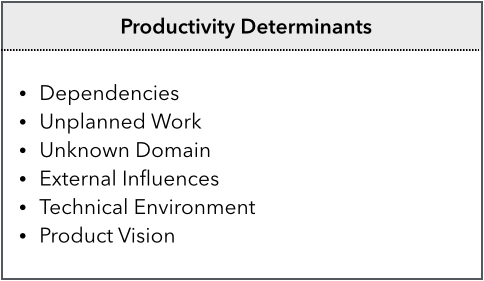
\includegraphics[width=0.50\textwidth]{figures/productivity-determinants.png}
  \caption{Productivity determinants}
  \label{fig:productivity-determinants}
\end{figure}

\begin{description}

   \item[Dependencies.] Providing the development teams with independent work packages, on which \acp{XFT} can focus during their sprints is  desirable. However, such an isolation of work is hard to achieve in an organisation where many teams are working on several products. As noted by the interviewees, it is not uncommon to be interconnected in one way or another with other parts of the organisation. Namely, there is a need to coordinate with another unit in the organisation while working on the first step of some user stories, where a meeting should be booked and prepared for, thus demanding a noticeable amount of communication.

      %\begin{quote}\itshape Many of our stories are actually that we should book a meeting, we should have that meeting in the week or something like that and we need to do some preparation sometimes...
      %\end{quote}

   Another perspective on dependencies is related to more implementation level, where being dependent on progress of others can cause stalling or, if dependencies are not communicated properly and remain hidden, it can ultimately lead to complete invalidation of work effort.

      %\begin{quote}\itshape It could be some delivery that is delayed or something like that.
      %\end{quote}

   %If the dependencies remain hidden, it can ultimately lead to complete invalidation of work effort:

      \begin{quote}\itshape... one team is doing work in the same area of the code and they don’t know about someone else is doing a delivery and suddenly everything that you have made is not valid anymore because it doesn’t align with what has just been delivered in.
      \end{quote}

However, discovered dependencies are readily discussed and collaborated on between developers, but tend to cause more intense communication between \acp{XFT} than usual, as heat maps \emph{Resolving technical dependencies} on Figure \ref{fig:hm-r} depict. Both heat maps show a high communication intensity around the \quotes{\ac{XFT} Developers} and \quotes{XFT Scrum Masters} indicated by the respective cells in the heat maps being of high values corresponding to the shades of red on a colour key, and at least three distinct roles being the communication's target.

\begin{figure}[h!]
   \makebox[\textwidth]{%
      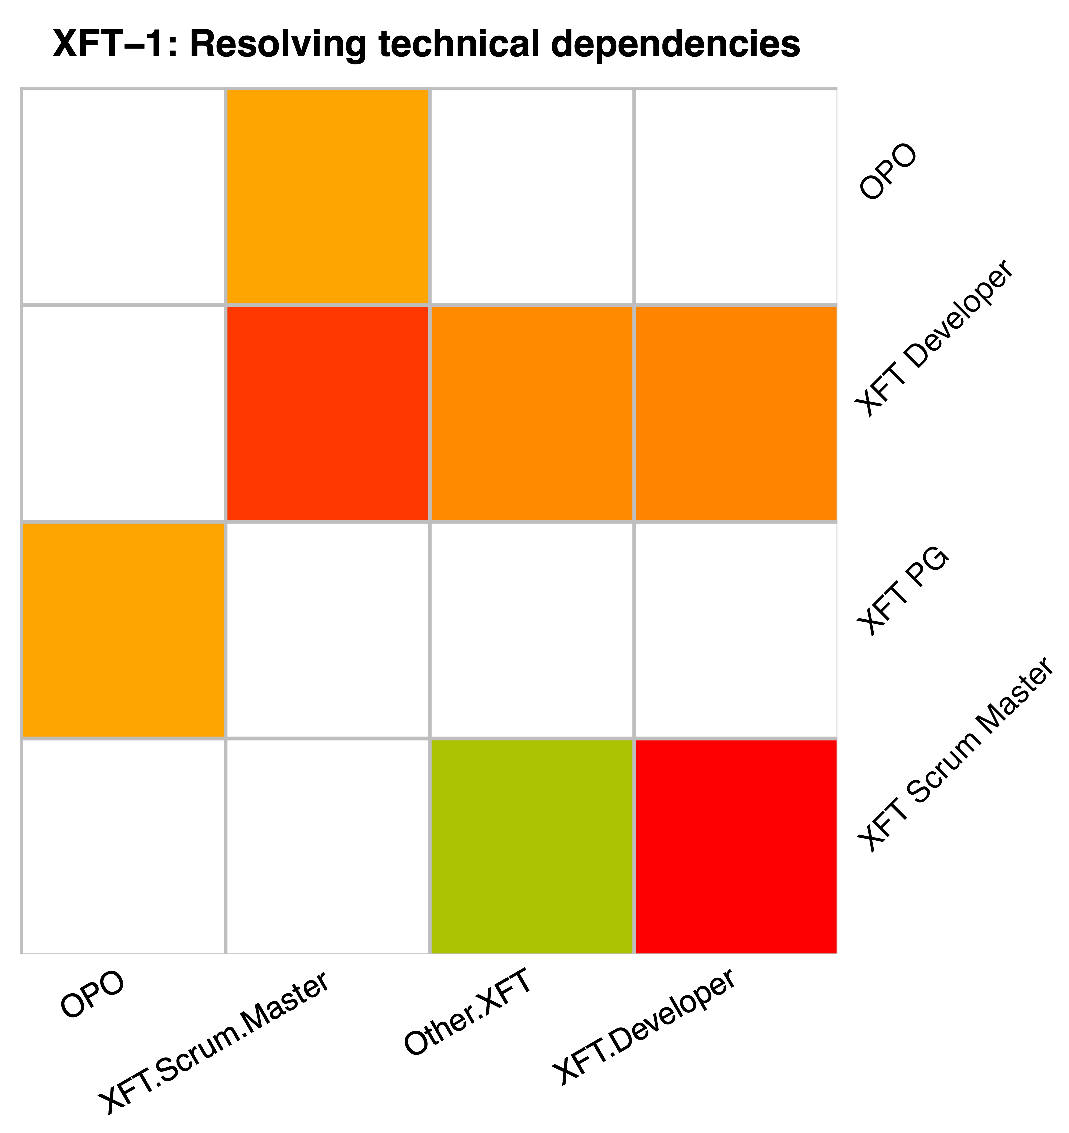
\includegraphics[width=0.45\textwidth]{figures/heatmaps/ms2-_r_.pdf}%
      \hfill    
      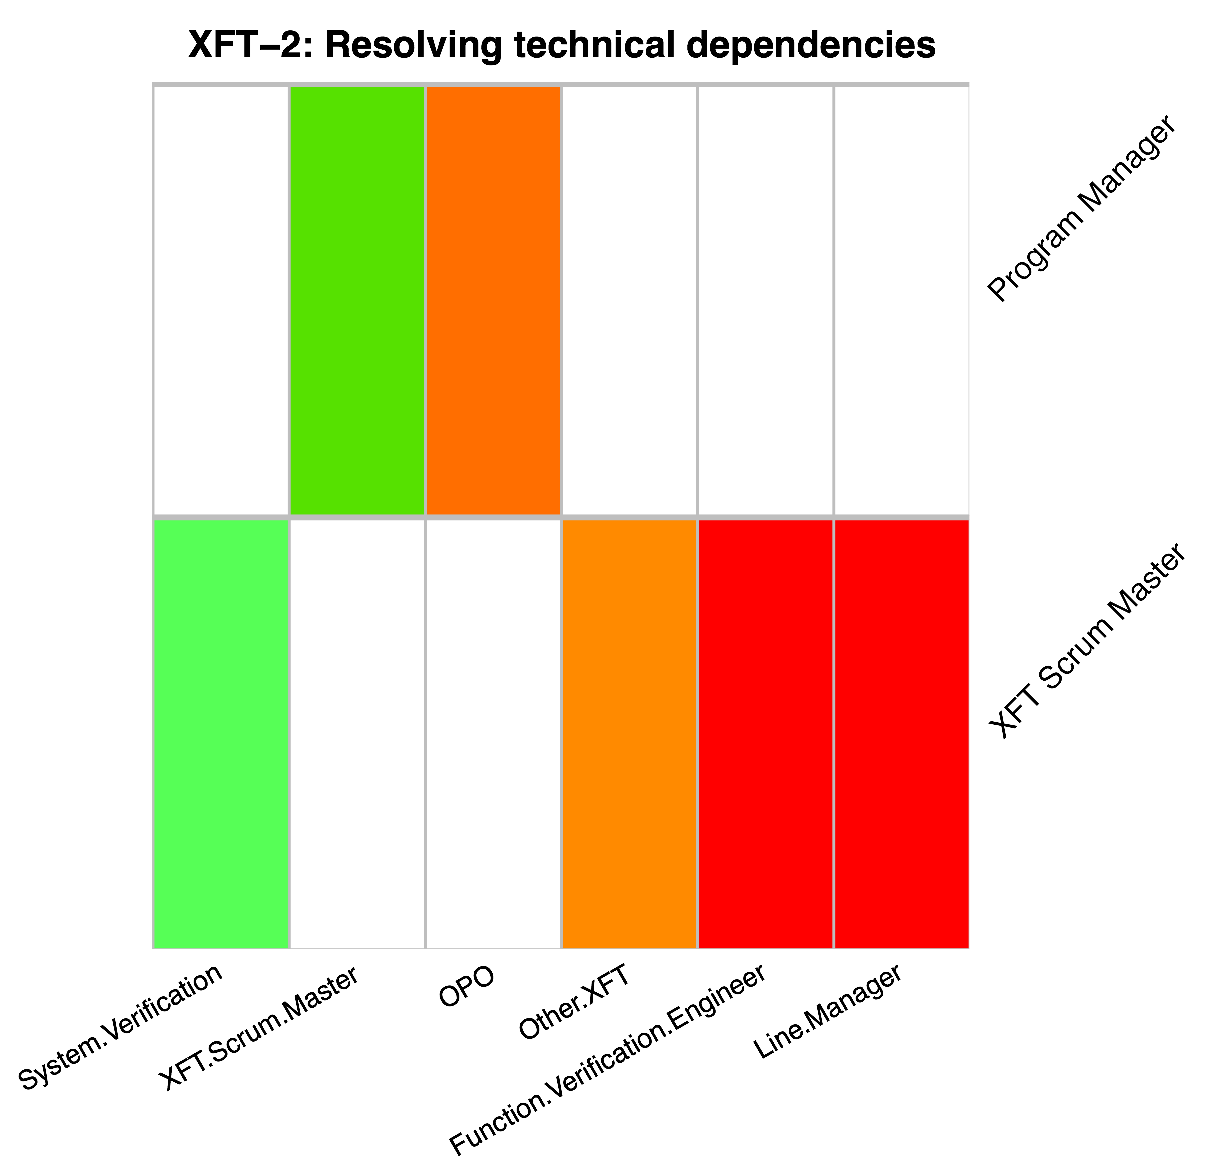
\includegraphics[width=0.49\textwidth]{figures/heatmaps/picnic-_r_.pdf}%
   }
      \caption{Heat maps: resolving technical dependencies}
      \label{fig:hm-r}
\end{figure}

In addition to this, the social networks in the Figures \ref{fig:ms2-sn} and \ref{fig:picnic-sn} demonstrate a quite significant amount of contacts for the \acp{XFT} with entities outside their immediate environment within a week long period.

    \item [Unplanned Work.] The commitment to a set of stories throughout the duration of a sprint, as considerably emphasized in Scrum, is not always strictly followed by the studied organisation. \acp{XFT} experience influences from different parts of the organisation, which do not necessarily contribute to the progress of development. In this regard, it is noted that the teams get additional stories from the line organisation, which do not contribute to the work on a product, but are intended to help the line organisation to get better integrated with the remaining elements of the structure.

%      \begin{quote}\itshape... they get some quite a few small extra tasks to help the line get into the organisation. I think it takes some time from the team.
%      \end{quote}

   Aside from additional tasks, developers are often disturbed by the trouble reports which can be put forward by customers or fellow development teams. In case of a high severity a report may force an \ac{XFT} to put the ongoing stories aside to fully concentrate on the report at hand:

      \begin{quote}\itshape... that started up as a small TR that someone started to work on and the suddenly it got really, red alert on it, so everything within Ericsson was almost stopped because this TR must be solved. And then of course, at least two of the teams were involved at the same time and it took one week to solve it.
      \end{quote}

   These items of unplanned work being pushed in to the backlog ultimately affect the teams' velocity by shifting the focus of developers. As reported, assigning a single team member to a trouble report often entails eventual involvement of additional person due to severity of a report or lack of competence. One of the interviewed XFT members recalls weeks where the work on a backlog has been completely set aside as every team member was dealing with trouble reports.

%      \begin{quote}\itshape ...that person who looks into or answers that question or looks into that problem might need to ask someone else in a team for help and then you have two people working on that. We had weeks where we had three problems and we were all working on that and work has stopped on the planned work.
%      \end{quote}
      
Communication intensity-wise, however, such occurrences do not seem to cause more friction than the regular backlog work, as heat maps \emph{Backlog work on planned sprint goals} and \emph{Unexpected change or interruption} on Figure \ref{fig:hm-b-u} demonstrate. \emph{Unexpected change or interruption} heat maps show communication intensities for \quotes{XFT Developer} and \quotes{XFT Scrum Master} with shades of green colour codes indicating intensities below the usual level. This is similar to the communication nature of backlog work, where only in the case of the \quotes{XFT Developers} of the XFT-1 intensity slightly increases which is reflected with colour changing to orange.

\begin{figure}[h!]
   \makebox[\textwidth]{%
      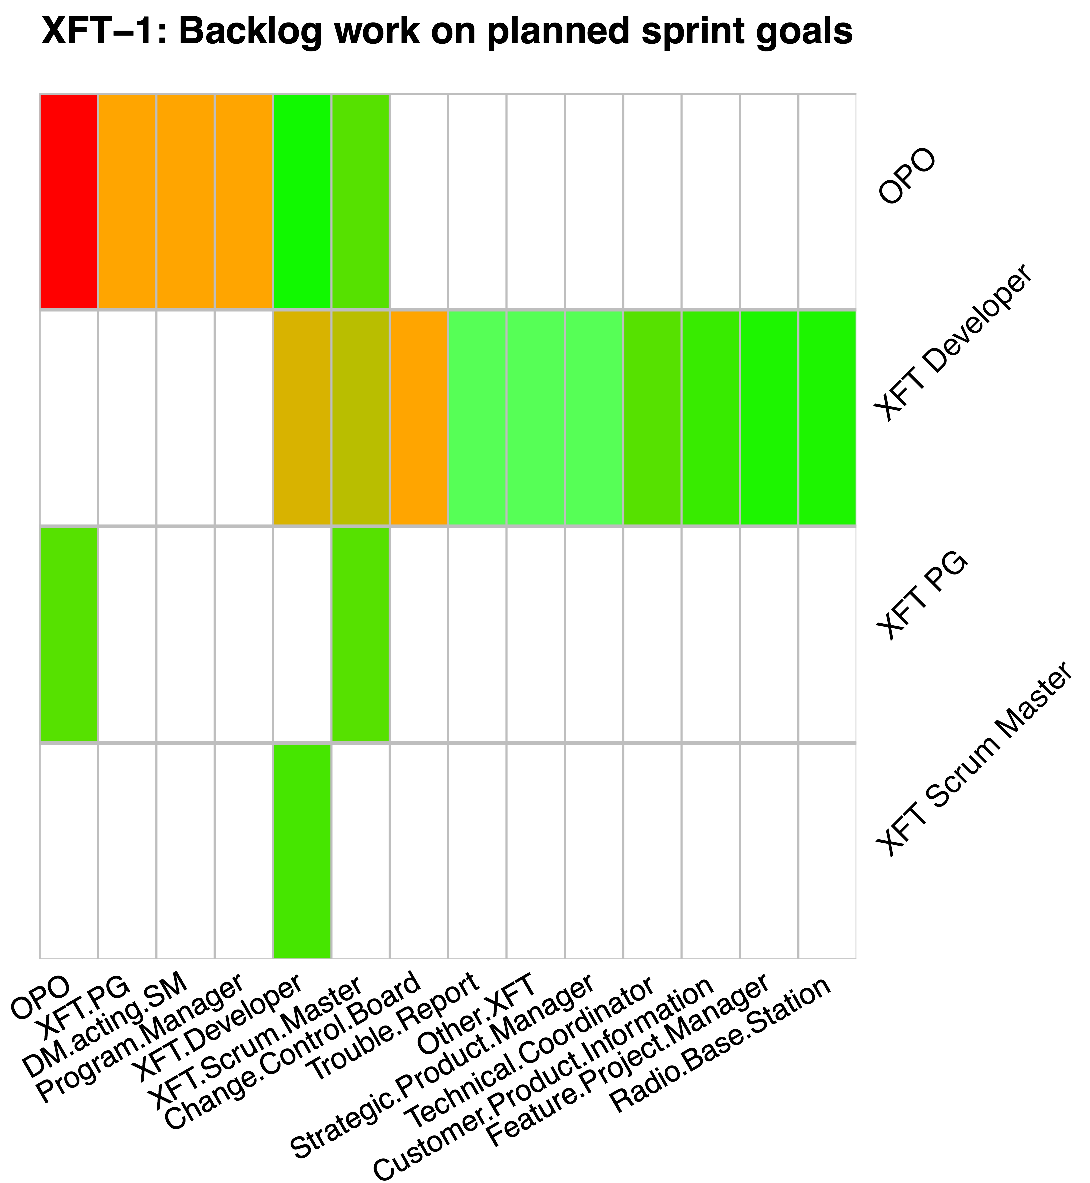
\includegraphics[width=0.44\textwidth]{figures/heatmaps/ms2-_b_.pdf}%
      \hfill    
      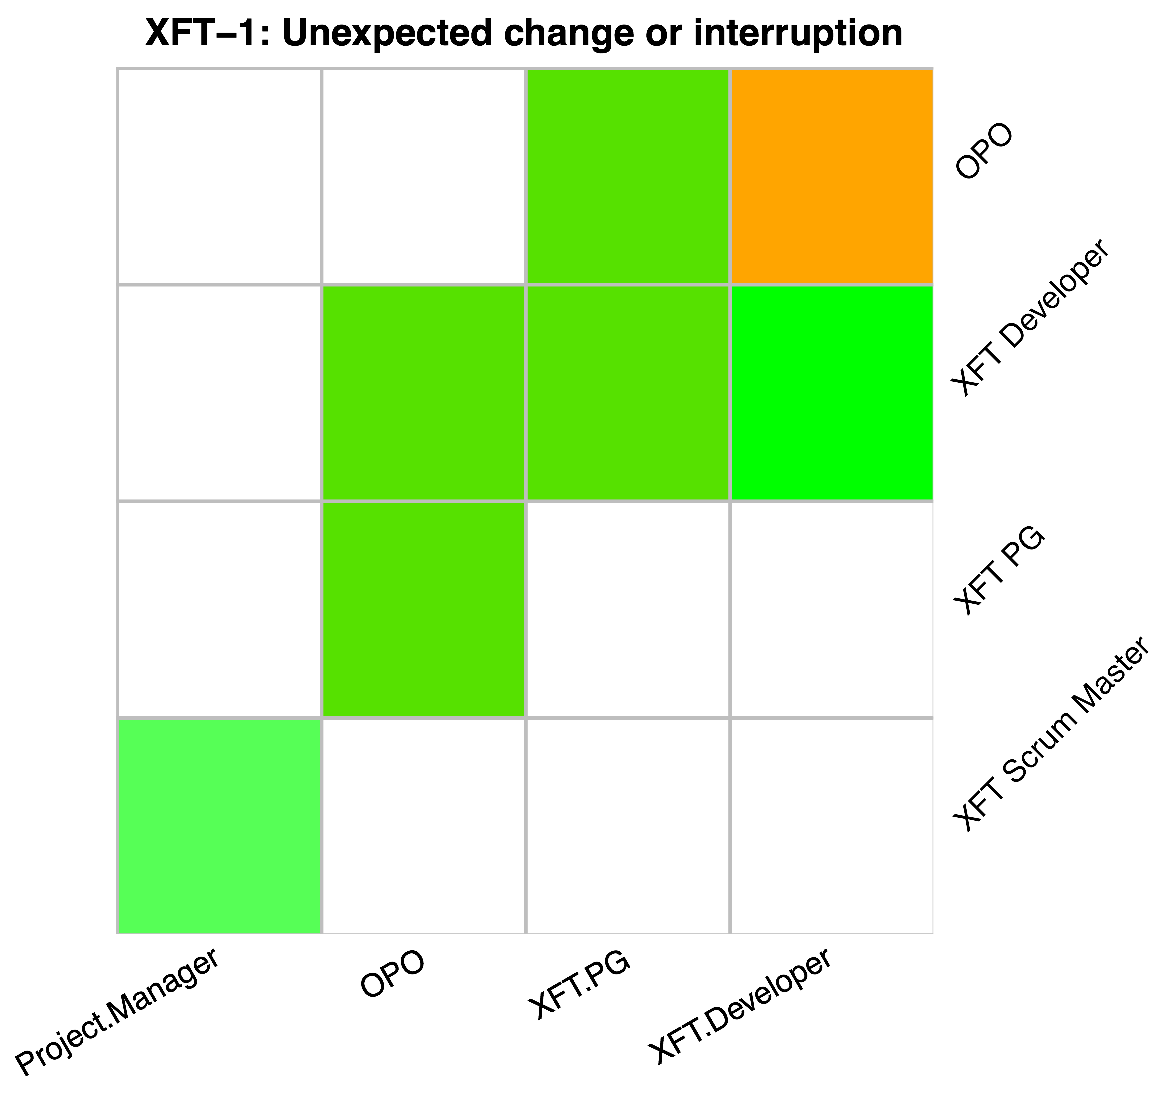
\includegraphics[width=0.49\textwidth]{figures/heatmaps/ms2-_u_.pdf}%
   }\\[0.5cm]% If you want some vertical space
   \makebox[\textwidth]{%
      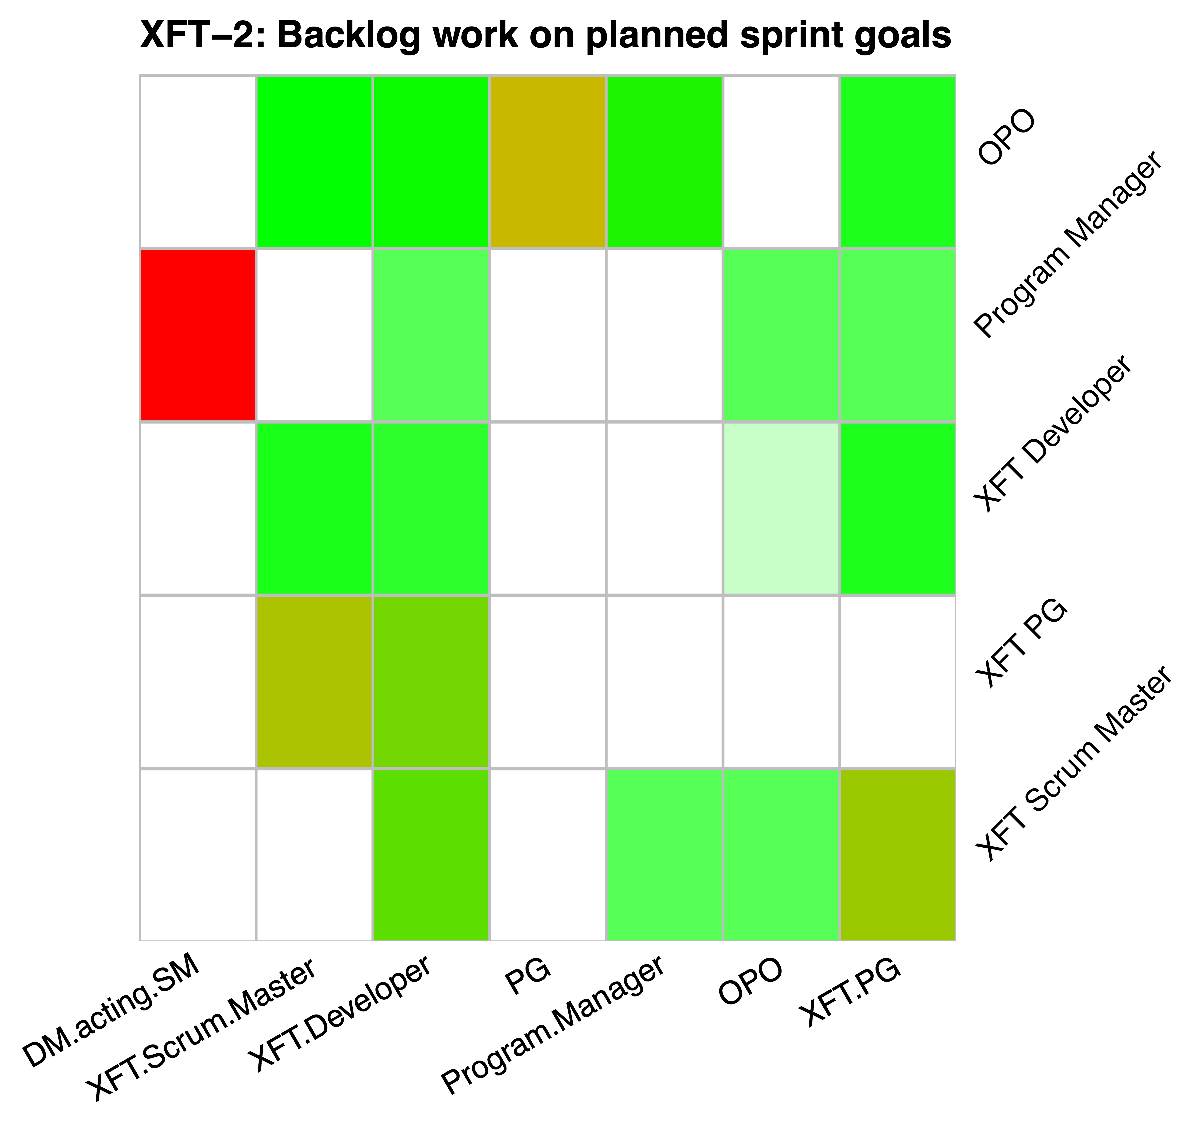
\includegraphics[width=0.49\textwidth]{figures/heatmaps/picnic-_b_.pdf}%
      \hfill    
      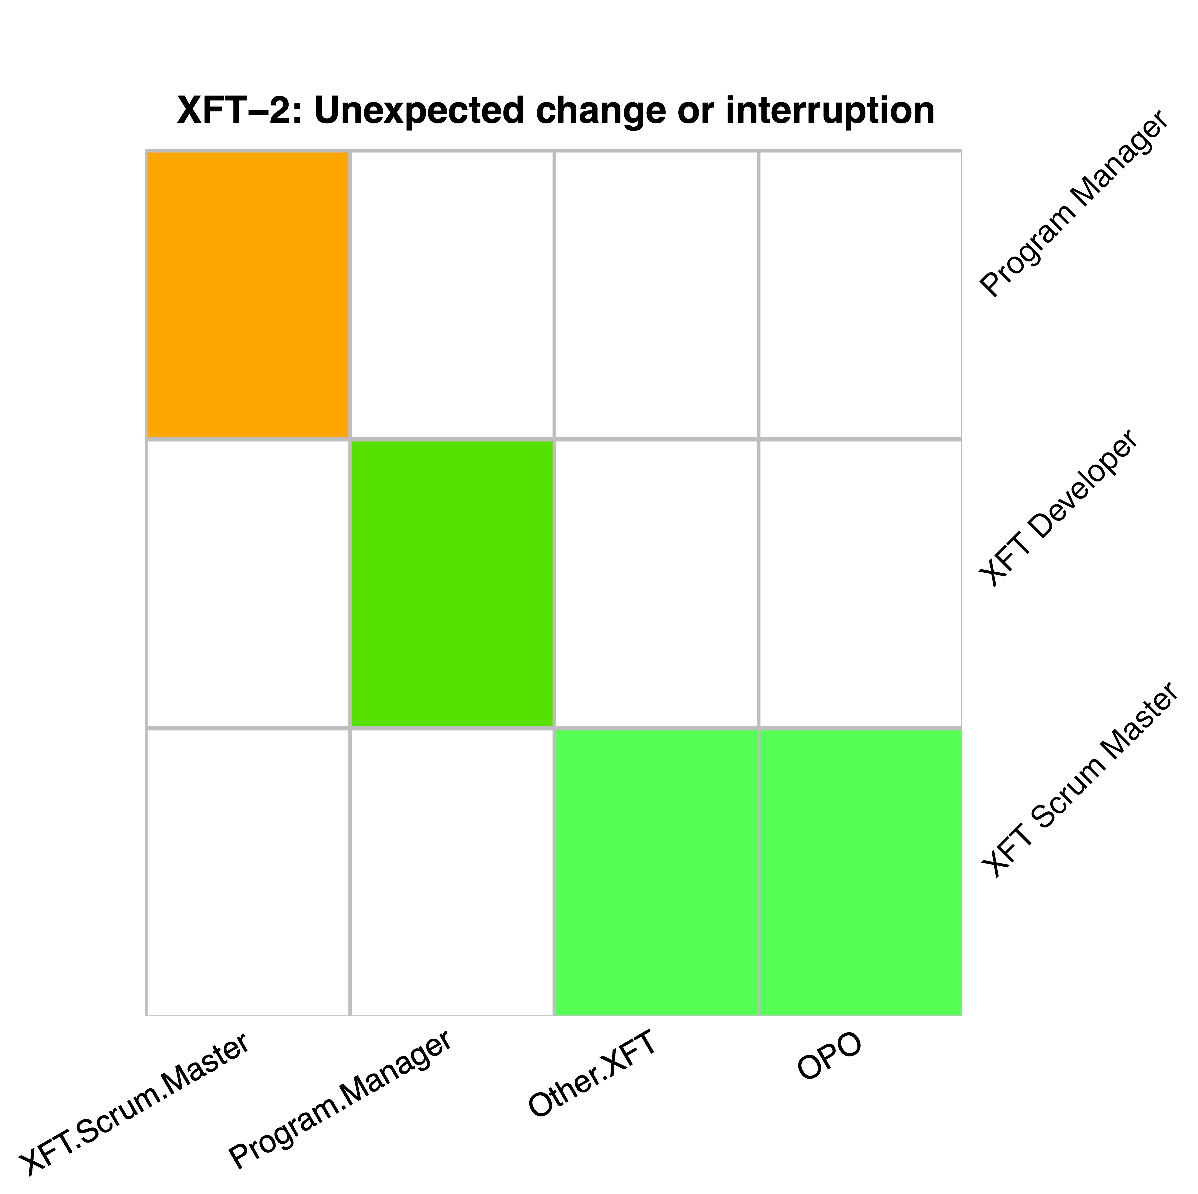
\includegraphics[width=0.49\textwidth]{figures/heatmaps/picnic-_u_.pdf}
      }
      \caption{Heat maps: backlog work and unexpected change}
      \label{fig:hm-b-u}
\end{figure}

    \item [Unknown Domain.] The \acp{XFT} in the studied organisation are encouraged to take on tasks from different product areas. This sometimes causes teams to work in areas out of their expertise within an unknown domain. Familiarisation with the new area demands tremendous effort prior to actual development.

      \begin{quote}\itshape ... we spend days just on getting to know their code and so on, because it's said that we should do all development, but... Yes, we could do it, but it takes several days more than if we just ask someone who knows this from the beginning.
      \end{quote}

   In addition, variety of work packages disrupts the sense of a single purpose inside the team.

   \item [External Influences.] Shielding \acp{XFT} from external influences and disruptions enables them to retain focus on backlog work and thereby positively affects the burn-down. Interviewees however note outside factors crawling into their daily work and distracting them from backlog items. One example is an urgent re-prioritisation of tasks that might be the result of a management decision.
    
%      \begin{quote}\itshape... it’s normally due to urgent re-prioritisation of the work. Something has happened that is unexpected.
%      \end{quote}

   Another case is forced participation in events which might not affect \acp{XFT} directly, and from the XFT members' perspective the things discussed in such meetings are not relevant for their sprints. The time spent is thus viewed as waste.

%      \begin{quote}\itshape... because they discuss things that are not relevant for my sprint or my team and then I think it is waste.
%      \end{quote}

   Alternatively, such events can be beneficial as they concern teams' future work, but the effect of that influence is only experienced by the teams in a number of months in the future.

      \begin{quote}\itshape ... we have lots of other meetings that show up suddenly, some pre-study that starts and we really need to attend that one because we going to work with that in 2 months
      \end{quote}

    \item [Technical Environment.] One of the issues having its origins in the \acp{XFT}' empowerment is concerned with their technical environment. Empowering the XFTs means providing them with control over the great part of it. At the same time, such delegation of responsibilities is not necessarily beneficial, as the teams might not have the competence required to take care of the variety of arising issues. In this regard the interviewees repeatedly reported on being stalled by factors outside of their responsibility or competence.
    
      \begin{quote}\itshape So that has taken a lot of time and that, if you need a node and you are dependant on the nodes and you run a command and you need the traces, your work stops and that's what we have not gotten help with and we still do not know how to do that.
      \end{quote}

    \item [Product Vision.] The organisation's magnitude and its structure with several layers between developers and customers diminished the notion of customer collaboration. Thus, teams tend to have little participation in product discussions. At the same time, the wish of a long-term product vision being communicated to teams has been brought up. It could bring \acp{XFT} closer to customers and motivate their work which in turn could positively affect product quality. As of now, the vision is not being communicated to the teams to a desirable extent, potentially rooted in the fact that those with more customer contact have perspective rather different from the teams'.

   Moreover, those with a vision are faced with its agility and fragility and thus do not communicate it fully as it might change at any moment:

      \begin{quote}\itshape I think they like to know what we will go, the goals, but in this agile world, I think, it’s sometimes it will just change again, even if we have this plan.
      \end{quote}

   However, in some of the respondents' opinion, the vision's carriers may sometimes be not passing it along due to lack of personal interest and involvement.

%      \begin{quote}\itshape If I should speak for myself, I don't think [the Product Owner] is that interested in the [product], to have that vision for [product].
%      \end{quote}
   
%   All in all, it would help \acp{XFT} to be more motivated and gain more influence upon a given product.
   
%      \begin{quote}\itshape I think it would be more fun, because then we could actually have more input on the product, because then we would have some general vision on what we are about to develop in the future.
%      \end{quote}
      
In the case of the \ac{XFT}-1 the \ac{APO}'s role has the most customer contact among all roles present in the network in the Figure \ref{fig:ms2-apo}, but there is no direct link between the two. It proves how problematic the establishment of tighter collaboration between the customer or through their \ac{PO} representative and the team members can be. As of now the communication has to travel via two intermediates: an \ac{OPO} and a \ac{PgM}. Referring back to the diagram on Figure \ref{onion}, it does not alight with the intended collaboration.

\begin{figure}[h!]
  \centering
  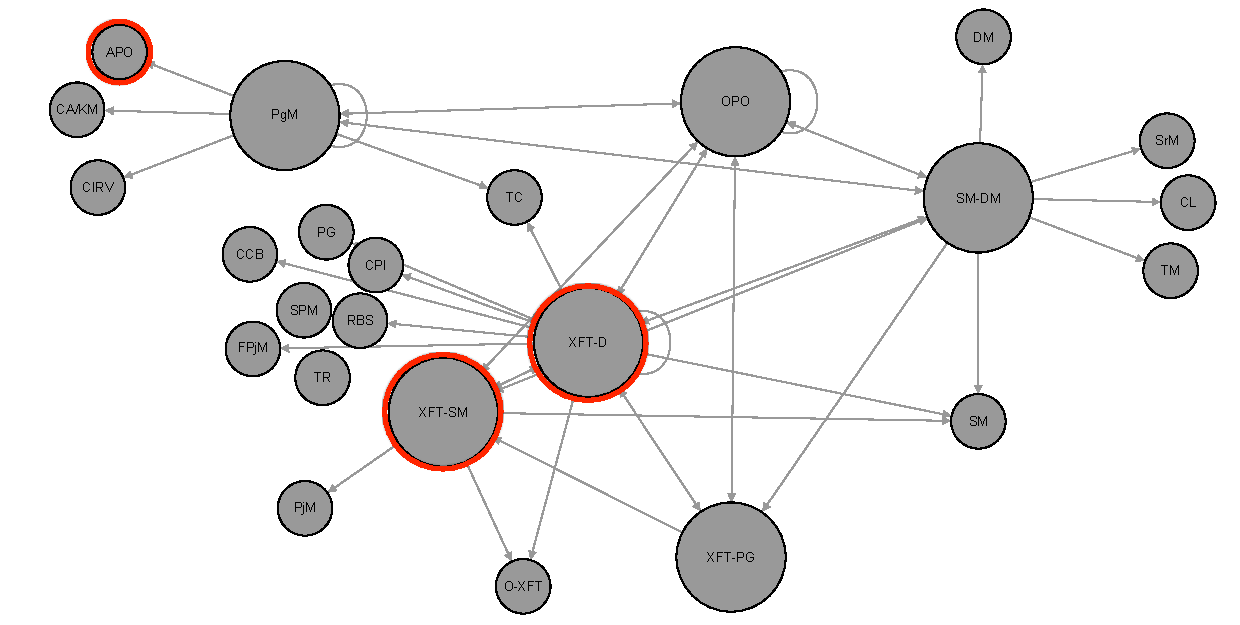
\includegraphics[width=0.8\textwidth]{figures/ms2-apo.pdf}
  \caption{XFT-1: contact with APO}
  \label{fig:ms2-apo}
\end{figure}

\end{description}
